% options:
% thesis=B bachelor's thesis
% thesis=M master's thesis
% czech thesis in Czech language
% hidelinks remove colour boxes around hyperlinks

\documentclass[thesis=M,czech]{FITthesis}[2019/12/23]

\usepackage{graphicx} %graphics files inclusion
\usepackage{dirtree} %directory tree visualisation
\usepackage{minted}
\usepackage{xevlna}
\usepackage{csquotes}
\usepackage{pdflscape} % lscape pokud se nema otacet stranka
\usepackage{bookmark} % pro moznost ukonceni part
\usepackage[style=iso-numeric]{biblatex}

\usemintedstyle{xcode} % aby nebyly zvyrazneny chyby v Reactu (minted neumi JSX) TODO
\addbibresource{sources.bib}
\setcounter{biburllcpenalty}{7000} % aby se spravne lamaly adresy v bibliografii:
\setcounter{biburlucpenalty}{8000}
\setcounter{tocdepth}{3} % nadpisy vsech urovni v obsahu
\definecolor{bg}{rgb}{0.95,0.95,0.95} % pozadi pro kody
\renewcommand{\listingscaption}{Ukázka kódu}
\renewcommand{\listoflistingscaption}{Seznam ukázek kódu}

% % % % % % % % % % % % % % % % % % % % % % % % % % % % % % 
\department{Katedra softwarového inženýrství}
\title{Rozšíření webové aplikace pro projekt \enquote{Úspěšný prvňáček}}
\authorGN{Lukáš} %(křestní) jméno (jména) autora
\authorFN{Rod} %příjmení autora
\authorWithDegrees{Bc. Lukáš Rod} %jméno autora včetně současných akademických titulů
\author{Lukáš Rod} %jméno autora bez akademických titulů
\supervisor{Ing. Stanislav Kuznetsov}
\acknowledgements{Rád bych poděkoval Ing. Stanislavu Kuznetsovi za cenné rady a pomoc při tvorbě této práce. Děkuji za spolupráci své mamce, PaedDr. Janě Rodové, která se mnou jakožto lektorka Úspěšného prvňáčka po celou dobu spolupracovala. Děkuji celé své rodině a přátelům za podporu a trpělivost během celého studia.}

\abstractCS{...} %TODO

\abstractEN{...} %TODO

\placeForDeclarationOfAuthenticity{V~Praze}
\declarationOfAuthenticityOption{1} %volba Prohlášení (číslo 1-6)

\keywordsCS{webová aplikace, Úspěšný prvňáček, Python, Django, React, Django REST framework} %TODO
\keywordsEN{web application, Successful first-grader, Python, Django, React, Django REST framework} %TODO
\website{https://github.com/rodlukas/masters-thesis} %volitelná URL práce, objeví se v tiráži - úplně odstraňte, nemáte-li URL práce
% % % % % % % % % % % % % % % % % % % % % % % % % % % % % % 

\begin{document}
    
    \begin{introduction}
    	Proces vývoje jakékoliv aplikace nikdy nekončí a jinak tomu není ani v případě současné webové aplikace pro projekt \enquote{Úspěšný prvňáček}\footnote{\url{https://uspesnyprvnacek.cz/}} (dále jen ÚP) vedený speciální pedagožkou PaedDr.~Janou Rodovou. Uplynuly přesně dva roky od nasazení první produkční verze v rámci mé bakalářské práce. Tomu předcházela dlouhá cesta příprav, analýz, rešerší, návrhů a poté implementace. Cesta to byla trnitá, i díky volbě mně naprosto cizích nejmodernějších technologií pro serverovou i klientskou část, snaze o jejich propojení, někdy nepříliš přívětivé dokumentaci či odlišným přístupům frameworků. Vše se ale nakonec zdárně podařilo a po akceptačním testování a posledním vyladění lektorka mohla spokojeně začít aplikaci každodenně používat. Existence této aplikace znamenala obrovský skok kupředu vzhledem k tomu, že do té doby byl užíván pro část evidence naprosto nedostačující Microsoft Excel, pro část klasický diář a pro další část různé papíry. To vše díky aplikaci skončilo.

Na závěr bakalářské práce jsem uváděl možná rozšíření v budoucnu, a to nezůstalo jen u slov. O měsíc později po odevzdání bakalářské práce naplno začala druhá etapa vývoje aplikace. O této etapě budu psát v rámci celé této diplomové práce. Během tohoto necelé dva roky trvajícího postupného vývoje bylo třeba řešit mnoho \enquote{kostlivců}, mnoho chyb, o kterých jsem v době vytváření neměl ani tušení. Ale také mnoho nových funkcí, protože bylo potřeba jít kupředu vzhledem k rozvoji samotného ÚP. Jak vývoj postupoval, přicházely další a další nové výzvy, požadavky a poznání. Objevilo se také několik slepých uliček. Ale nebudu předbíhat.

U projektu ÚP jsem již od samého počátku, a proto je tato webová aplikace mou srdeční záležitostí. Mojí snahou bylo tedy vyhovět naprosto všem požadavkům lektorky tak, aby s každou novou verzí byla její práce hladší, jednodušší a efektivnější. Další motivací je možnost si v rámci tohoto vývoje vyzkoušet další řadu nových technologií, nástrojů a přístupů a zdokonalit se tak v oblasti tvorby moderních webových aplikací.

V teoretické části nejprve stručně popíši, co nabízí původní verze aplikace vypracovaná v rámci bakalářské práce -- jaké má funkce, použité technologie, jak funguje nasazování a do jakých prostředí se nasazuje. Zmíním zde i stručně původní náměty na rozšíření aplikace do budoucna, o kterých bylo uvažováno na závěr bakalářské práce. Poté se zaměřím na rešerši možností automatizovaného testování webových aplikací a možných nástrojů pro usnadnění vývoje a údržby. Na závěr zvolím vhodné technologie a nástroje pro tuto práci a volbu oargumentuji.

V praktické části nejprve provedu sběr a analýzu požadavků a navrhnu úpravy včetně aktualizovaného databázového modelu a upraveného schéma API (Application Programming Interface). Poté již popíši postupně všechny kroky v rámci implementace všech požadavků a zavedení nástrojů. Následovat bude podrobný popis vytváření testů, které budou tvořit důležitý podpůrný prvek celého vývoje a popis nového způsobu nasazování aplikace včetně konfigurace více prostředí. Na závěr uvedu možná rozšíření aplikace v budoucnu a také popíši kroky učiněné pro zveřejnění aplikace jako open-source.
    \end{introduction}
    
    \chapter{Cíle práce}
        TODO \cite{test}
    
    \part{Teoretická část}
        \chapter{Aktuální řešení}

V této kapitole stručně popíši verzi aplikace, která byla vytvořena v rámci bakalářské práce \cite{bp} a kterou budu v praktické části rozšiřovat. Popíši implementované funkční i nefunkční požadavky, použité technologie a také konfiguraci prostředí a způsob nasazování. Na závěr stručně shrnu, jaké možné plány na rozšíření byly v rámci bakalářské práce nastíněny.

\section{Implementované požadavky}

\subsection{Implementované funkční požadavky}

V této podsekci shrnu implementované funkční požadavky. Součástí této podsekce je také původní logický datový model aplikace z bakalářské práce \cite{bp} na obrázku~\ref{fig:db-model} pro lepší pochopení domény.

Shrnutí funkčních požadavků \cite{bp}:
\begin{itemize}
    \item \textbf{evidence klientů:} evidování základních informací o klientovi,
    \item \textbf{evidence lekcí klientů:} evidování základních informací o lekcích (včetně stavů účasti všech účastníků a stavu jejich platby za danou lekci), lekce mohou být pro jednotlivce nebo pro skupiny, každá náleží nějakému kurzu,
    \item \textbf{evidence předplacených lekcí:} předplacená lekce je řešená jako lekce, která nemá datum a čas konání,
    \item \textbf{evidence kurzů a stavů účasti:} pro použití při evidenci lekcí,
    \item \textbf{přehled lekcí pro aktuální den:} zobrazení pro dnešní lekce (kromě zrušených),
    \item \textbf{karta klienta a skupiny}: zobrazení všech informací o klientovi/skupině včetně všech lekcí,
    \item \textbf{upozornění na platbu příště:} když už klient nemá žádné předplacené lekce, zobrazí se u poslední placené lekce upozornění na fakt, že má příště zaplatit,
    \item \textbf{pořadové číslo lekce:} u lekce se zobrazí (automaticky vypočítáno), o kolikátou navštívenou lekci v pořadí se jedná,
    \item \textbf{týdenní přehled:} zobrazení lekcí jako v diáři.
\end{itemize}

\begin{figure}[h]\centering
	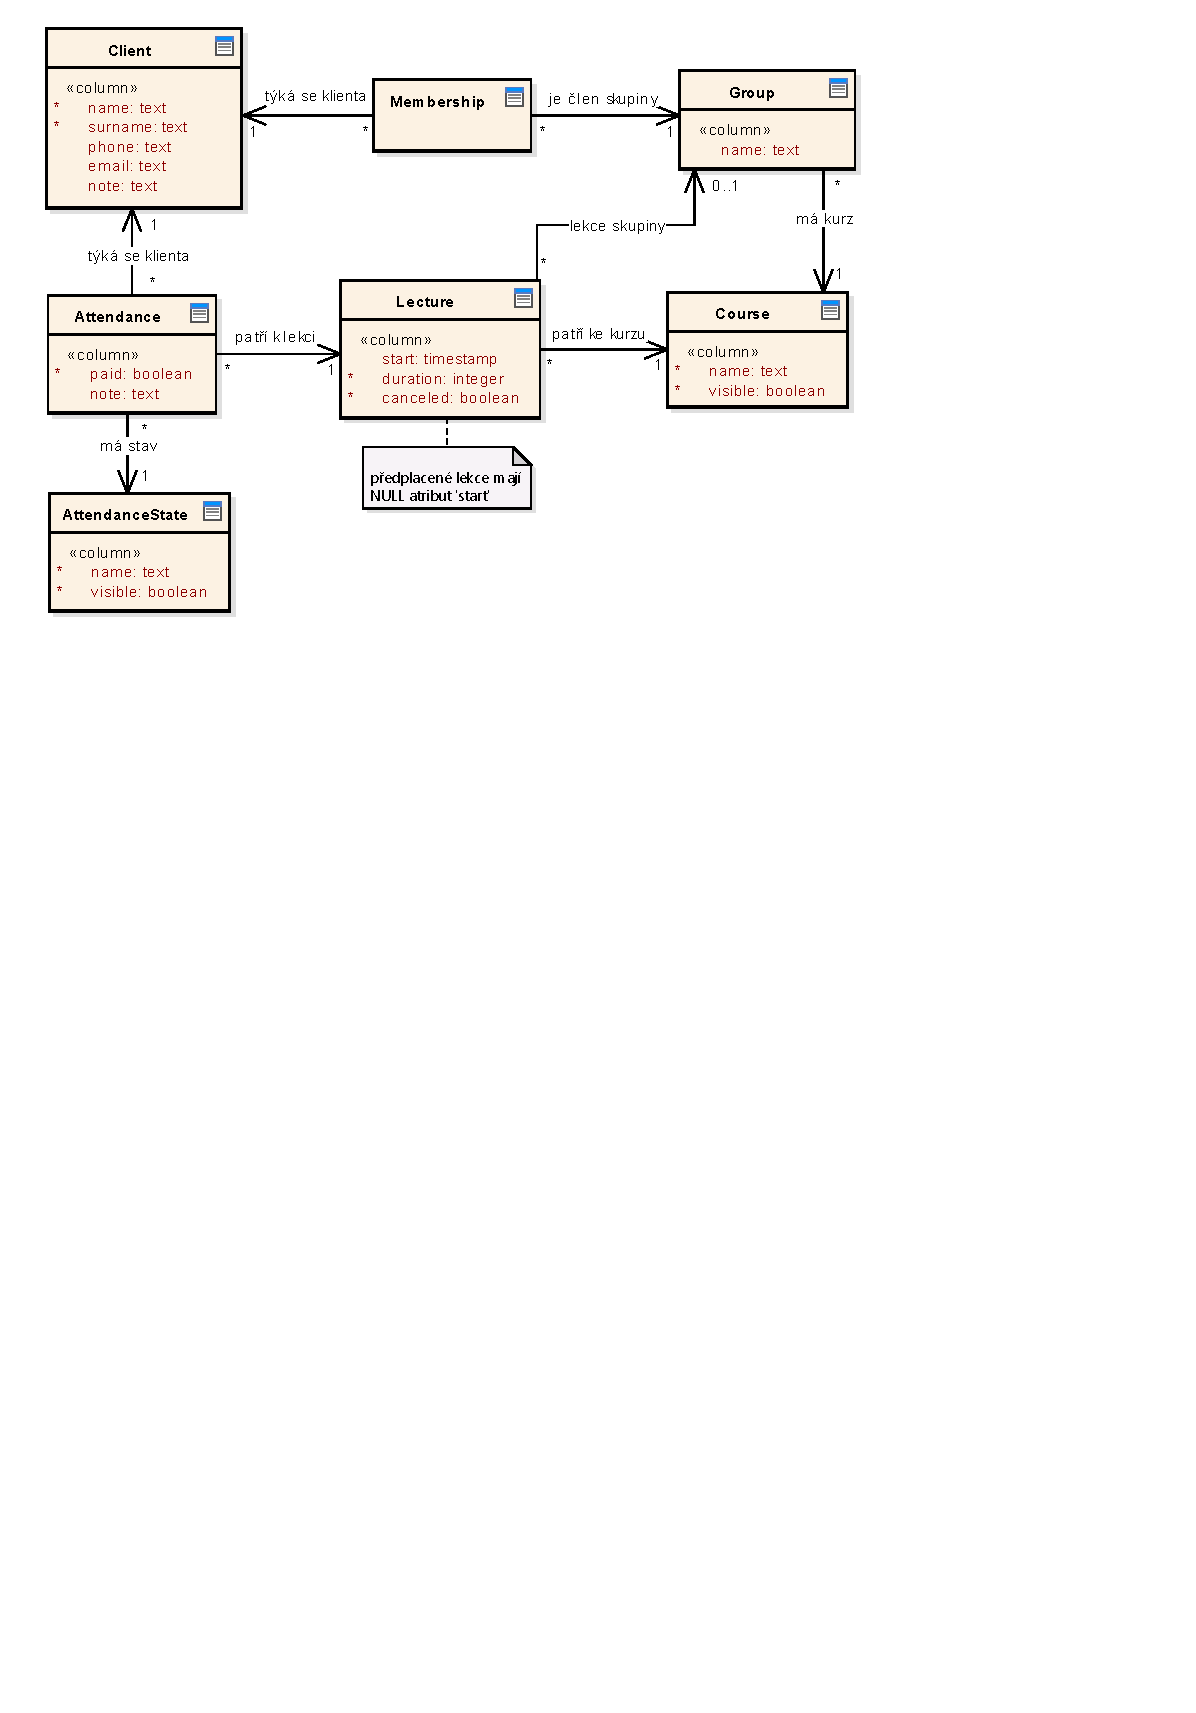
\includegraphics[width=1\textwidth]{img/bp/db-model}
	\caption[Logický datový model z bakalářské práce]{Logický datový model z bakalářské práce \cite{bp}}\label{fig:db-model}
\end{figure}

\subsection{Implementované nefunkční požadavky}

Následuje shrnutí nefunkčních požadavků \cite{bp}:
\begin{itemize}
    \item \textbf{kompatibilita s webovými prohlížeči:} aplikace je plně funkční a kompatibilní s běžnými webovými prohlížeči (Google Chrome, Mozilla Firefox, Microsoft Edge, Apple Safari) v posledních verzích, důraz je především kladen na desktopový prohlížeč Mozilla Firefox, na kterém se aplikace používá primárně,
    \item \textbf{podpora široké škály zařízeních:} aplikace je responzivní a korektně se zobrazuje na všech zařízeních používaných lektorkou -- iPad s iOS~13.3 a 9,7palcovým displejem, Nokia~5 s Androidem~9.0 a 5,2palcovým~displejem, notebook s Windows~10 s rozlišením 1920~×~1080 a 15,6palcovým~displejem,
    \item \textbf{připravenost na rozšíření a údržbu}: kód byl tvořen s důrazem na budoucí možná rozšíření (např. použití konstant, respektování principu DRY (\enquote{Don\textquotesingle t repeat yourself}) ad.),
    \item \textbf{bezpečnost:} JWT (JSON Web Token) autentizace a další produkční konfigurace pro zabezpečení aplikace,
    \item \textbf{srozumitelné a jednoduché rozhraní aplikace:} iterativní návrh a implementace UI za neustálé spolupráce s lektorkou pro dosažení co nejlepší použitelnosti.
\end{itemize}


\section{Použité technologie}

\subsection{Serverová část}

Serverová část aplikace \cite{bp} je napsána v Pythonu~3.6.5 s webovým frameworkem \href{https://www.djangoproject.com/}{Django~2.0.5}. Pro správu závislostí se používá pouze jednoduchý soubor \verb|requirements.txt| obsahující specifikace přesných verzí knihoven (bez povolení jakkoliv malých aktualizací). 

Aplikace vystavuje REST~API postavené na frameworku \href{https://www.django-rest-framework.org/}{Django~REST~framework~3.8.2}. Na produkci se používá webový server \href{http://gunicorn.org/}{Gunicorn~19.8.1} spolu s knihovnou \href{http://whitenoise.evans.io/en/stable/}{WhiteNoise~3.3.1} pro efektivní servírování zkomprimovaných statických souborů \cite{whitenoise}.

\subsection{Klientská část}

Klientská část aplikace \cite{bp} je napsána v JS (JavaScript) ve standardu ECMAScript®~2018 a čistém CSS (Cascading Style Sheets). Pro správu závislostí se používá soubor \verb|package.json|, v němž jsou verze přibližně poloviny knihoven definovány napevno (bez možnosti jakkoliv malé aktualizace), druhá polovina knihoven přijímá malé aktualizace. 

Klientskou část aplikace lze klasifikovat jako: 
\begin{itemize}
    \item \textbf{SPA} (Single-Page Application), tedy aplikaci běžící přímo u klienta v prohlížeči nevyžadující znovunačítání při přecházení mezi stránkami \cite{spa1} a
    \item \textbf{CSR} (Client-Side Rendering), tedy aplikaci, která je klientovi doručena jako jednoduchý HTML (Hypertext Markup Language) soubor s odkazy na JS/CSS (Cascading Style Sheets) soubory \cite{csr-ssr}.
\end{itemize}

Je postavena na knihovně \href{https://reactjs.org/}{React~16.3} spolu s UI frameworkem \href{https://getbootstrap.com}{Bootstrap~4.1} a související knihovnou \href{https://reactstrap.github.io/}{Reactstrap~5.0}, která umožňuje jednoduché použití Bootstrap komponent v Reactu \cite{reactstrap}. Pro asynchronní požadavky na REST API využívá knihovnu \href{https://github.com/axios/axios}{axios~0.18}. 

Konfigurace celé klientské části stojí na nástroji \href{https://github.com/facebook/create-react-app}{create-react-app~1}, který umožňuje \cite{cra} vytvářet React aplikace bez počáteční konfigurace. Vzhledem k použití Djanga bylo ale potřeba \cite{bp} pomocí příkazu \verb|eject| \enquote{vysunout} celou konfiguraci klientské části a pomocí knihoven \href{https://github.com/owais/webpack-bundle-tracker}{webpack-bundle-tracker} a  \href{https://github.com/owais/django-webpack-loader}{django-webpack-loader} propojit Django s nástrojem Webpack. Webpack zde umožňuje mj. spouštět vývojový server pro klientskou část a vytvářet z jednotlivých modulů klientské části balíčky, které lze pak po zadaných transformacích servírovat na produkci pro běžné webové prohlížeče \cite{webpack-ackee}.

V případě vývoje na lokálním stroji se používá \cite{bp} pro serverovou část vývojový Django server a pro klientskou část \href{https://github.com/webpack/webpack-dev-server}{webpack-dev-server}, oba nabízejí podporu pro \enquote{hot reloading} (tedy okamžité automatické projevení změn v kódu bez kompletního znovunačtení aplikace \cite{webpack-docs-hmr}) a v tomto ohledu bylo vše i díky zmíněným knihovnám zprovozněno.

\section{Prostředí, testování a nasazování}

Aplikace \cite{bp} je verzována v privátním repozitáři na serveru GitHub. Při každém nahrání nové revize na server (\verb|push|) se na integračním serveru \href{https://travis-ci.com/}{Travis~CI} spustí sestavení aplikace, vytvoří se testovací databáze a spustí se základní testy (viz níže). Výsledné pokrytí kódu spočítané pomocí nástroje \href{https://coverage.readthedocs.io/}{Coverage.py} se poté nahraje na platformu \href{https://codecov.io/}{codecov.io} pro pokročilé statistiky o testování \cite{codecov}. Pokud vše na Travisu proběhne v pořádku, začne nasazení na produkční server běžící na \href{https://www.heroku.com/}{Heroku}. Nasazení na Heroku probíhá tak, že se přímo na něm spouští celé sestavení aplikace znovu, zmigruje se databáze a aplikace se nasadí. I tento průběh lze sledovat přímo z Travis terminálu.

Spouštěné testy jsou základní a velmi jednoduché, otestují \cite{bp}:
\begin{itemize}
    \item přidání klienta a uživatele do databáze přes Django modely,
    \item zda Django uživateli zobrazí správnou stránku při příchodu do aplikace (neřeší, zda se pak vůbec JS aplikace vyrenderuje),
    \item funkčnost API požadavků -- proběhne autorizace (a tedy získání JWT tokenu) a pokus o vytvoření nového klienta přes API.
\end{itemize}

Jak je vidět, testy byly skutečně pouze velmi povrchní, dalo by se říci, že se jedná o smoke testy. Také je třeba zdůraznit, že provedení \verb|push| na repozitář mělo za následek okamžité nasazení na produkci, pokud sestavení a tyto základní testy prošly. To může být nedozírné následky. I proto se v dalších kapitolách této teoretické části budu zaobírat možnostmi zlepšení.

\section{Plán rozšíření z bakalářské práce}

Na závěr bakalářské práce \cite{bp} bylo zmíněno několik možných rozšíření aplikace. Následuje jejich přehledný stručný přehled, v kapitole~\ref{pozadavkyanalyza} se mimo jiné na některá z nich také dostane.

Přehled možných rozšíření \cite{bp}:
\begin{itemize}
    \item \textbf{vylepšení předplacených lekcí:} pohodlnější způsob zaznamenávání předplacených lekcí, pro skupiny je to velmi krkolomné a nepohodlné, pro jednotlivce také,
    \item \textbf{kontrola časového konfliktu lekcí:} aby se dvě nezrušené lekce vzhledem k datumu, času a délce trvání nijak nepřekrývaly,
    \item \textbf{vyhledávání v aplikaci:} např. vyhledávání klientů,
    \item \textbf{evidování zájemců o kurz:} pro plánování nových lekcí kurzů pro jednotlivce a skupiny,
    \item \textbf{evidence pomůcek a učebnic},
    \item \textbf{testy:} doplnění dalších testů a vysoké pokrytí kódu,
    \item \textbf{migrace na nový React:} k vydání verze 16.3 došlo na konci vývoje aplikace v rámci bakalářské práce, např. došlo ke změnám v API (životní cyklus komponent) \cite{react-blog-163},
    \item \textbf{React Context API:} analýza možností využití Context API v rámci nového Reactu \cite{react-blog-163}, zejména by pravděpodobně pomohlo snížit např. počet přístupů do API z klientské části napříč aplikací,
    \item \textbf{offline přístup:} analýza možností řešení offline přístupu, např. automatické ukládání do Google kalendáře, progresivní webové aplikace apod. a s tím související další oblasti jako SSR (Server-Side Rendering) -- tedy klient obdrží od serveru HTML dokument připravený k vyrenderování, oproti CSR, kde by klient pro vyrenderování aplikace musel čekat na stažení a spuštění JS souborů \cite{csr-ssr}.
\end{itemize}

\chapter{Možnosti automatizovaného testování}

Testování je důležitou součástí softwarového vývoje \cite{test-bdo}. V této kapitole nejprve srovnám manuální a automatizované testování, poté se zaměřím na strukturu samotných testů -- do jakých vrstev se dělí a kolik testů by v těchto vrstvách mělo být. Některé metodiky softwarového vývoje jsou zaměřené na způsob testování, proto uvedu hlavní principy těchto metodik a s nimi související nástroje, které umožňují tyto metodiky zavést. Uvedu i další nástroje pro testování UI.

\section{Srovnání manuálního a automatizovaného testování}
Dříve, když trval vývojový cyklus několik měsíců až let, se obvykle testovalo převážně pouze manuálně \cite{test-kitner}. Tedy na základě scénářů testeři prováděli testy \cite{test-bdo}. Dnes, v době agilního vývoje a rychlých dodávek, je potřeba větší část testování provádět automatizovaně \cite{test-kitner}. Tedy naprogramovat testy a poté je automaticky spouštět testovacím nástrojem \cite{test-bdo}. Díky tomu se týmy mohou dozvědět o chybě v řádu sekund a minut místo dnů a týdnů \cite{test-fowler}.

\textbf{Výhodou} automatizovaného testování je:
\begin{itemize}
    \item šetří čas, je rychlejší, umožní rychleji vydávat nové verze (kompletní manuální testování bylo úzkým hrdlem v životním cyklu vývoje softwaru) \cite{test-kitner, test-genez, test-cd},
    \item odhalí chyby v dřívějších fázích, tedy snižuje náklady \cite{test-kitner},
    \item dělá testování \enquote{zábavnější} a umožní efektivnější manuální testování -- odstraňuje běžnou neustále opakující se rutinu při manuálním testování \cite{test-kitner, test-perfecto},
    \item dochází ke zpřesnění testů a vyšší spolehlivosti, protože se tester při neustálém opakování na všech operačních systémech a prohlížečích může splést nebo něco přehlédnout \cite{test-kitner, test-genez},
    \item možnost vyššího pokrytí kódu testy a odhalení více chyb díky jednoduchému zavedení více permutací různých zařízení a operačních systémů \cite{test-perfecto},
    \item umožňuje zavést průběžnou integraci a dodávání \cite{test-kitner2}.
\end{itemize}

\textbf{Nevýhodou} automatizovaných testů je:
\begin{itemize}
    \item při nesprávném rozhodnutí o oblasti, kterou budeme optimalizovat, můžeme stovky hodin strávit při vytváření testů, které nakonec nebudou vůbec nacházet podstatné chyby \cite{test-kitner},
    \item nevhodně napsané testy mohou dát falešnou naději, že vše funguje, ačkoliv se v aplikaci vyskytují závažné chyby \cite{test-devqa},
    \item nikdy zcela nenahradí lidské pozorování (při manuálním testování) a nemohou garantovat přívětivost k uživateli či pozitivní uživatelský prožitek \cite{test-genez},
    \item vyšší pravděpodobnost falešně pozitivních výsledků, následná analýza problému je náročná, protože je třeba zjistit, zda se jedná o chybu aplikace či testu \cite{test-perfecto},
    \item nutnost neustálé údržby testů -- při zavedení změny v aplikaci je třeba vše co nejdříve (ideálně okamžitě) projevit do testů \cite{test-swsrovnani}.
\end{itemize}

Jak je vidět ze shrnutí výhod a nevýhod automatizovaného testování, manuální testování má v softwarovém vývoji stále své místo. Zejména kvůli lidskému faktoru a v případech, kdy se konkrétní test nemá spouštět opakovaně kvůli časové náročnosti vytvoření automatizovaného testu \cite{test-bdo}. Na možnosti aplikace manuálního a automatizovaného testování lze také nahlížet z hlediska různých testovacích cyklů softwaru \cite{test-bdo}, tedy manuální testování je vhodné na počátku vývoje/iterace a na závěr při testech použitelnosti, kde je důležitý lidský faktor. Automatizované testování je pak vhodné pro fázi testování výkonu a také pro fázi regresních testů \cite{test-bdo}, ty se využívají při opětovném testování stávajících funkcí a vlastností aplikace při provádění změn, například rozšiřování jiných oblastí či opravě chyb \cite{test-regresni}. Jak uvádí \cite{test-bdo}, je třeba nalézt pomyslný \enquote{rovnovážný bod}, který reprezentuje optimální poměr manuálních a automatizovaných testů vzhledem k ceně jejich vytvoření a počtu běhů testu -- cena vytvoření automatizovaného testu je vysoká, pokud poběží jednou, ale rychle se snižuje s počtem opakování, naproti tomu manuální testování je levné, ale s každým během se cena zvyšuje kvůli délce běhu testu.

Díky vytvoření automatizovaných testů lze aplikaci průběžně testovat na integračním serveru při každé revizi \cite{test-kitner}, to umožní ještě rychlejší zpětnou vazbu, rychlejší vydávání verzí a spokojenost zákazníka \cite{test-perfecto}. Aplikace je totiž prakticky připravená na nasazení v každé revizi \cite{test-atlassian}.

\section{Struktura automatizovaných testů}

Automatizované testování prostupuje více úrovněmi softwarového projektu \cite{test-kitner2} a je důležité na počátku tvorby testů stanovit, kde se bude automaticky testovat \cite{test-kitner}. Jednou z častých strategií zejména agilních týmů je strategie tzv. \enquote{testovací pyramidy} \cite{test-smartbear}. V této sekci tuto strategii představím a popíši, jak se dle různých zdrojů aplikuje, zaměřím se také na další alternativní přístupy.

\subsection{Testovací pyramida}

Testovací pyramida rozděluje automatizované testy do několika oblastí \cite{test-smartbear}, viz obrázek~\ref{fig:testing_pyramid}. Popis pyramidy vychází z \cite{test-kitner2, test-smartbear}. Obvykle by měly být jádrem automatizovaných testů unit testy, které ověřují, zda jednotlivé dílčí části kódu odpovídají požadavkům. Těchto testů by měla být většina. Následují testy komponent (např. přihlášení uživatele, tvorba účtu, objednávky) a integrační testy (ověří, že jednotlivé komponenty spolu interagují tak, jak bylo zamýšleno, např. data zákazníka jsou napříč celým procesem objednávky korektně přenášena). Jak je vidět na obrázku~\ref{fig:testing_pyramid}, vrstvy nejsou pevně definované a často některé splynou v jednu \cite{test-fowler}. Pod vrcholem pyramidy se nalézají API testy a na vrcholu jsou UI testy (někdy nazývané end-to-end, funkční či e2e), které by měly typicky mít nejmenší podíl ze všech automatizovaných testů vzhledem k jejich náročnosti na tvorbu a křehkosti při změnách UI. Mimo pyramidu, případně na úplný vrchol lze pak zařadit samotné manuální testy UI.

\begin{figure}[ht]\centering
	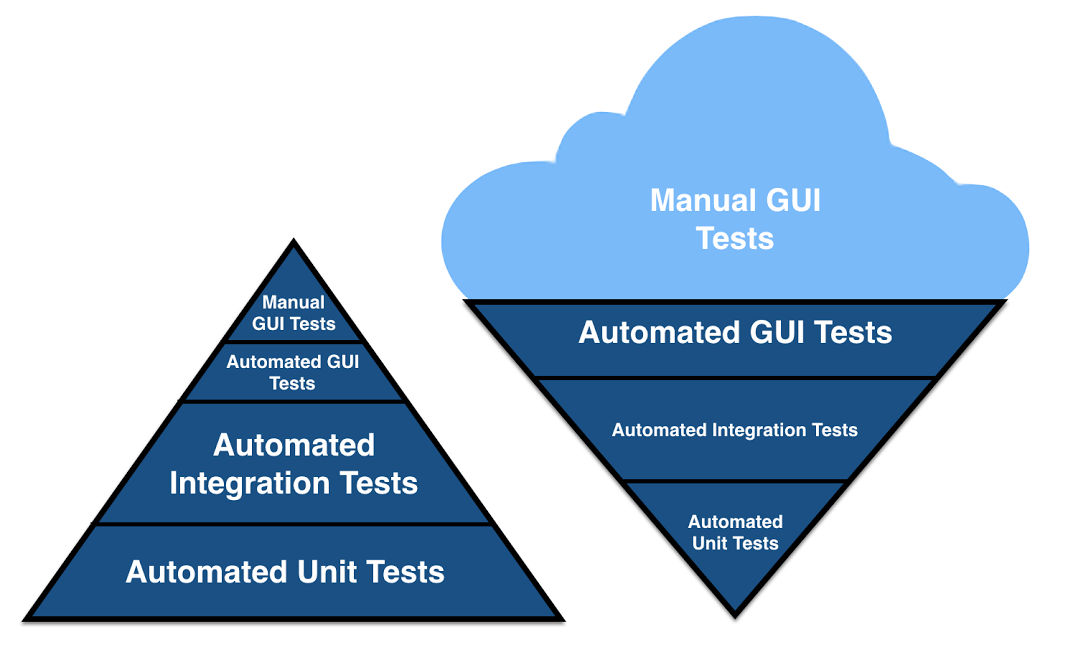
\includegraphics[width=1\textwidth]{img/ext/testing_pyramid.png}
	\caption[Srovnání strategie \enquote{testovací pyramidy} a \enquote{zmrzlinového kornoutu}]{Srovnání strategie \enquote{testovací pyramidy} (vlevo) a \enquote{zmrzlinového kornoutu} (vpravo) \cite{test-fishman}}\label{fig:testing_pyramid}
\end{figure}

Konkrétní aplikace této strategie závisí na vlastnostech projektu, týmu a požadavcích. Přesto se pokusím uvést obecná doporučení různých autorů. Čím níže z pohledu test pyramidy se podaří vývojářům dostat, tím lépe pro budoucí práci -- lépe začít např. s API, než s UI -- případně lze pracovat ve více lidech na více úrovních paralelně \cite{test-kitner}. Pokud ale aplikace už běží a postrádá jakékoliv testy, je ideální začít s tvorbou testů na vrcholu pyramidy pro kritické klíčové části byznysu \cite{test-atlassian}. Pro zbytek je vhodné využít nižší úrovně testů \cite{test-atlassian2}.

Mnoho organizací má i přes testovací pyramidu většinu automatizovaných testů postavených nad UI vrstvou \cite{test-devqa}, výhodou je dohled nad výsledným produktem, který je pak používán, nevýhodou křehkost a nesnadné dohledávání původu chyb zachycených při testech UI, v případě použití AJAX (Asynchronous JavaScript and XML) je také mnohem složitější vytvořit deterministické UI testy \cite{test-timothy}. Testovací pyramida je pak obrácená a obvykle se tomuto přístupu vzhledem k tvaru obrácené pyramidy říká \enquote{zmrzlinový kornout} \cite{test-mf1}, viz opět obrázek~\ref{fig:testing_pyramid}. 

Při volbě správné části k testování je třeba řídit se tím, která část je pro byznys zákazníka důležitá \cite{test-kitner}, než pouze například co nejvyšším pokrytím kódu testy \cite{test-devqa}. V případě, že se UI testy použijí pro klíčové funkce aplikace, můžeme zajistit, že i přes případné drobnější chyby funguje ta nejdůležitější část aplikace korektně, a to včetně všech vrstev jako např. napojení na API, databázi ad., to umožní častější dodávání nových verzí zákazníkovi s větší jistotou fungování, to vše je ale třeba dělat s vědomím jednotlivých úrovní testovací pyramidy a důsledků použití UI testů \cite{test-novanet}. Je tedy vhodné ve vyšší vrstvě testovat dva typy průchodů -- nejhorší a nejideálnější -- a pro zbytek hraničních případů využít vrstvy nižší \cite{test-dzone}.

Strategie testovací pyramidy je často špatně interpretována a může například vyústit v napsání naprosto všech možných unit testů a poté přesunutí do vyšší vrstvy atd., což pro některé týmy může být vhodné, pro jiné ale zbytečně komplexní a drahé \cite{test-cucumber2}. Principem pyramidy je naznačit, že testů na vyšší vrstvě má být méně než na nižší \cite{test-cucumber2}. Ačkoliv se princip testovací pyramidy stává standardem pro agilní týmy, je třeba rozumět principům, se kterými tento přístup přichází a na základě zavést způsoby testování pro konkrétní projekt \cite{test-cucumber2}. Na závěr je třeba říci, že veškeré zmíněné termíny, názvy a definice nejsou rigorózní a často panují různé názory např. na rozdělení testovací pyramidy, definici UI testování (někdy synonymum end-to-end testování, někdo nikoliv z toho důvodu, že UI lze testovat i pomocí unit testů) a mnoho dalšího, při tvorbě testů v rámci softwarového produktu je tedy vždy třeba jasně vymezit a definovat rozsah testů, sjednotit terminologii a na všem se domluvit \cite{test-fowler}.

\subsection{Alternativní přístupy}

Alternativním přístupem pro testování klientské části je strategie tzv. \enquote{testovací trofeje} \cite{test-trophy}, která se skládá ze 4 částí, od té nejnižší: statické testy (založené na statickém typování a linterech, viz TODO), unit testy (cílené na kritické části aplikace), integrační testy (ověřující, že vše spolu korektně spolupracuje) a end-to-end funkční testy (simulace chování uživatele při důležitých průchodech aplikací prostřednictvím automatizovaného klikání -- tedy UI testy z testovací pyramidy). Jak ale opět uvádí \cite{test-roth}, tento přístup opět může pro některé týmy a aplikace být vhodný, pro některé nikoliv a bez dostatečné znalosti konkrétního kódu aplikace a problematiky může následování nejen tohoto vzoru vyústit ve slepou cestu.

\begin{figure}[h]\centering
	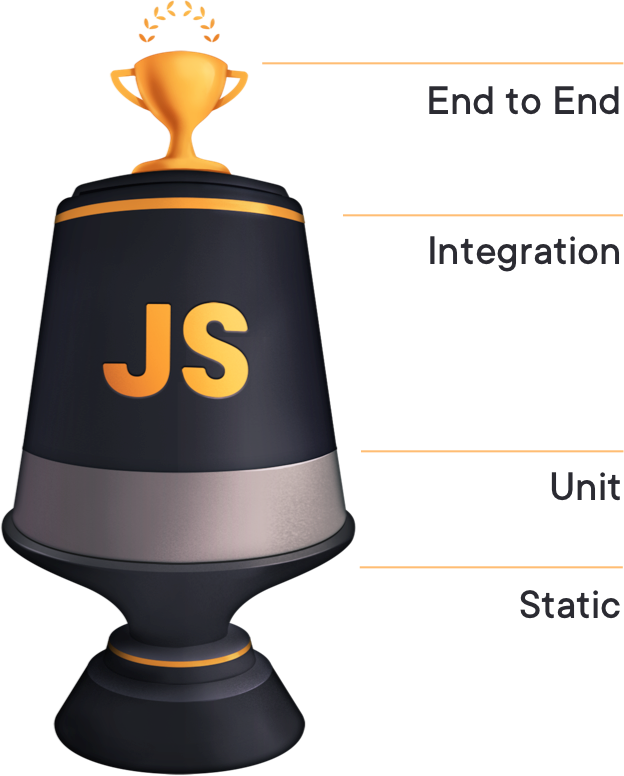
\includegraphics[width=0.4\textwidth]{img/ext/testing_trophy.png}
	\caption[Strategie \enquote{testovací trofeje}]{Strategie \enquote{testovací trofeje} \cite{test-trophy}}\label{fig:testing_trophy}
\end{figure}

\section{Metodiky a nástroje pro automatizované testování}

Svět testování je ovlivňován několika metodikami vývoje softwaru, především TDD (Test-Driven development) a BDD (Behaviour-Driven development) \cite{test-swtestinghelp1}. S těmito metodikami souvisí také různé nástroje pro automatizované testování podporující příslušný způsob vývoje, o nich se též zmíním. Na závěr uvedu ještě další nástroje pro UI testování.

\subsection{TDD}

Základním principem TDD je napsat nejprve testovací případy (přímo v programovacím jazyce) a až poté implementovat kód, který zařídí splnění těchto případů \cite{test-swtestinghelp2}. Výsledkem je vyšší kvalita a flexibilita kódu (tím pádem lze pak jednoduše provádět např. refaktoring) a také vysoké pokrytí kódu \cite{test-swtestinghelp2}. Nevýhodou TDD je, že změny ve fungování aplikace mohou mít velký dopad na testovací případy, testovacím případům také rozumí pouze lidé se znalostí programovacích jazyků \cite{test-swtestinghelp2}. Vzhledem k zaměření testů na konkrétní implementaci a nikoliv chování je ale snadnější najít v případě TDD testů konkrétní chybu  \cite{test-swtestinghelp2}. TDD testy se zaměřují zejména na nejnižší vrstvu v testovací pyramidě, tedy unit testy \cite{test-swtestinghelp1}, principy TDD se ale mohou aplikovat napříč všemi vrstvami \cite{test-dzone}.

Mezi nástroje pro podporu TDD patří xUnit frameworky, např. \href{https://junit.org/}{JUnit}, \href{https://testng.org/}{TestNG}, \href{https://nunit.org/}{NUnit} \cite{test-swtestinghelp2}. Pro JS se dle \cite{test-chart-js2} a \cite{test-chart-js1} nejvíce používá \href{https://jestjs.io/}{Jest} a \href{https://mochajs.org/}{Mocha}, pro Python se používá \href{https://docs.pytest.org/en/latest/}{PyTest} nebo \href{https://docs.python.org/3/library/unittest.html}{unittest} \cite{test-chart-python}.

\subsection{BDD}

BDD rozšiřuje TDD a místo psaní testovacích případů se zapisují požadované scénáře chování, později je opět implementován samotný kód aplikace zařizující její předem specifikované chování \cite{test-swtestinghelp2}. Díky zápisu scénářů v jazyce Gherkin, který vychází z přirozeného jazyka, je možná jednoduchá spolupráce mezi vývojáři, testery, analytiky a zákazníkem (i bez znalosti programovacích jazyků) \cite{test-swtestinghelp2, test-cucumber1}, vytvořené scénáře tvoří prakticky základ pro dokumentaci funkcí aplikace \cite{test-smartbear2}. Při vývoji aplikace totiž často dochází k nedorozuměním ohledně výkladu různých požadavků. Výhodou BDD je také zaměření na samotné chování aplikace, nikoliv na přemýšlení o implementaci v kódu, chování aplikace je hlavní prvek, na který se vývojáři a testeři zaměřují a umožňuje to tak držet se lépe požadavků zákazníka \cite{test-swtestinghelp2}. BDD testy se zaměřují zejména na prostřední vrstvy v testovací pyramidě, tedy API testy \cite{test-swtestinghelp1}.

Mezi nástroje pro podporu BDD patří frameworky jako \href{https://specflow.org/}{SpecFlow}, \href{https://cucumber.io/}{Cucumber}, \href{https://github.com/machine/machine.specifications}{MSpec} \cite{test-swtestinghelp2}. Ze scénářů lze vytvářet vždy aktuální dokumentaci a reporty díky nástrojům jako \href{https://smartbear.com/product/testcomplete/overview/}{TestComplete} \cite{test-smartbear2}. Pro JS se používá \href{https://cucumber.io/docs/installation/javascript/}{Cucumber.js}, pro Python se používá \href{https://behave.readthedocs.io/en/latest/}{Behave} \cite{test-chart-bdd}.

BDD se často používá spolu s TDD, protože dokáže na vyšší úrovni prověřit korektní fungování aplikace a poskytnout tak vyšší důvěru ve výsledný produkt \cite{test-cucumber1} -- takové testy tedy prověří nějaké chování aplikace a doplněním o TDD testy na nižších úrovních se dotestují specifické části.

\subsection{Další nástroje}

Jak jsem již zmínil, BDD se zaměřuje na vyšší vrstvy testovací pyramidy, pro UI testování se tedy často používá s nástroji jako \href{https://www.selenium.dev/}{Selenium} \cite{test-dzone}. Selenium je sada nástrojů a knihoven pro automatizované testování webových aplikací \cite{test-seleniumdocs}. Prostřednictvím tzv. WebDriveru, který je implementován jednotlivými tvůrci prohlížečů, umožňuje interagovat s webovou stránkou v prohlížeči (a to nejen v běžném módu, ale také tzv. \enquote{headless} módu, kde prohlížeč běží bez GUI) \cite{test-hackernoon1, test-seleniumdocs}. Pro \enquote{headless} mód byl do nedávné doby nejpopulárnější volbou \href{https://phantomjs.org/}{PhantomJS}, vzhledem k postupné implementaci této funkce do předních webových prohlížečů byl ale jeho vývoj zastaven a přechází ze na běžné prohlížeče, protože právě v těch koncový uživatel pracuje \cite{test-fowler, test-phantomjs}.

Selenium je mocný nástroj, nevýhodou je ale poměrně zdlouhavý zápis skriptů pro výběr elementů, práci s výjimkami a časováním, proto se často volí nádstavby zaobalující Selenium, které umožňují jednodušší zápis a práci, např. \href{https://selenide.org/}{Selenide} \cite{test-hackernoon1}. Také je možné využít komplexní testovací frameworky, které nabízí mnohem více nástrojů pro práci s testy, z nichž některé jsou také postavené na Seleniu, z mnohých používaných například \href{https://www.katalon.com/}{Katalon Studio} či \href{https://robotframework.org/}{Robot framework} \cite{test-selenium3, test-katalon}.

Selenium se postupem času stalo průmyslovým standardem pro UI testování, a to zejména díky jednoduchosti použití, kompatibilitě (s mnoha prohlížeči, možnost použití s mnoha programovacími jazyky) a popularitě \cite{test-selenium1}. Jak ale uvádí \cite{test-cypress1}, v případě asynchronních aplikací je Selenium složitější používat vzhledem k principu jeho fungování, protože je třeba vždy explicitně čekat na objevení elementu na stránce, problémem ale je, že nevíme, jak dlouho čekat. I z toho důvodu zde autor nabízí alternativu v podobě novějšího \href{https://www.cypress.io/}{Cypress}, který nabízí mnohem lepší práci s asynchronními aplikacemi, problémem ale je možnost použití pouze s JS, malá komunita a popularita, méně návodů \cite{test-cypress1}. Další nevýhodou Cypress byla podpora výhradně prohlížeče Google Chrome, to se ale v únoru 2020 změnilo \cite{test-cypress2}, naopak výhodou uváděnou např. v \cite{test-cypress3} byla lepší dokumentace oproti Seleniu, dokumentace Selenia ale byla kompletně přepsána a na podzim 2019 nasazena \cite{test-selenium2}.

\begin{comment}
% TODO?
\chapter{Konfigurace více prostředí}

tudle kapitolu možná nezařadím a rovnou popíšu způsob řešení v praktické části
obsah: Deployment environments a s tím související Release management

\begin{itemize}
\item přehled toho, jak se můžou řešit různý prostředí, např. staging, testing, produkce apod., asi se tomu rika deployment pipeline
\end{itemize}
\begin{itemize}
\item přehled toho jak s tím souvisí releasy, co kam může jít a k čemu je to dobrý, jak se to dá různě dělat a souvislosti (např. nemusí to dělat travis na základě releasu, ale třeba na základě podmínky proměnné prostředí nebo branch production apod.)f
\end{itemize}

viz:
\begin{itemize}
\item https://continuousdelivery.com/implementing/patterns/\#the-deployment-pipeline
\item https://en.wikipedia.org/wiki/Deployment\_environment
\item https://docs.gitlab.com/ee/ci/environments.html
\item https://cs.wikipedia.org/wiki/Release\_management
\item https://docs.microsoft.com/cs-cz/aspnet/web-forms/overview/deployment/configuring-server-environments-for-web-deployment/scenario-configuring-a-staging-environment-for-web-deployment
\item http://guides.beanstalkapp.com/deployments/best-practices.html
\item ...
\end{itemize}

\end{comment}

\chapter{Nástroje pro usnadnění vývoje a údržby}

Postupem času v rámci dalšího vývoje a rozšiřování aplikace se ukázalo, že je třeba použít pokročilé nástroje pro usnadnění samotného vývoje a údržby. Cílem této sekce je nastínit způsob jejich výběru. Jedním z hlavních požadavků je, aby vše potřebné bylo zdarma, neuvažuji zde tedy nástroje nenabízející alespoň nějakou formu bezplatného používání na dobu neurčitou (tedy nikoliv jen pro studenty). Při procházení ceníků budu brát také v úvahu fakt, že repozitář s projektem je open-source (to je jeden z cílů této práce). Při volbě nástrojů pro daný účel budou případně specifikovány další požadavky. Na základě průzkumu pak uvedu nalezené nástroje, jejich vlastnosti a seřadím je orientačně podle popularity na základě stránky \href{https://stackshare.io/}{StackShare}, která poskytuje \cite{stackshare} možnost sdílet používané nástroje a technologie firem a jednotlivců pro jejich projekty, nástroje a technologie srovnávat, hodnotit, řadit dle popularity apod.

\section{Monitorování chyb}
Pro každou aplikaci je důležité monitorovat chyby, díky tomu (nehledě na to, zda uživatel nahlásí problém a bude jakkoliv konkrétní) je možné pak chyby snadněji reprodukovat a opravit \cite{tools-exception}. Nástroje pro monitorování chyb umožňují upozornit vývojáře na výskyt chyby, poskytnout mu kompletní informace o chybě a kontextu, ve kterém nastala \cite{tools-exception}.

Minimální požadavky jsou:
\begin{itemize}
    \item zdarma pro použití na neomezenou dobu jak na Heroku (aplikace v rámci této práce), tak mimo Heroku (další aplikace např. v rámci ÚP) -- tento požadavek je zde kvůli existenci nástrojů jako např. \href{https://airbrake.io/}{Airbrake}, který na Heroku nabízí plán zdarma \cite{airbrake-heroku}, ale ve svém ceníku jej nenabízí \cite{airbrake-pricing}, tedy tyto nástroje neuvažuji,
    \item SaaS (Software as a Service) -- tedy aplikace hostovaná provozovatelem služby \cite{oracle-saas},
    \item možnost použití pro klientskou (JS s Reactem) i serverovou část (Python s Djangem).
\end{itemize}

Pro monitorování chyb existuje mnoho nástrojů, podle StackShare \cite{stackshare-exception} volím 4 nejpoužívanější, které splňují všechny požadavky. I přes mnoho dalších funkcionalit těchto nástrojů se zde zaměřuji na primární účel, tedy monitorování chyb -- nehledě na to, jaké další integrace a funkce jsou poskytnuty zdarma.

Nejpoužívanější nástroje podle StackShare (řazeno od nejpoužívanějšího) \cite{stackshare-exception} splňující zmíněné požadavky:
\begin{enumerate}
    \item \href{https://sentry.io/}{\textbf{Sentry}}: zdarma nabízí 5~000 událostí/měsíc pro neomezený počet projektů, 7~dní historie dat \cite{sentry-pricing}, podporuje React i Django \cite{sentry-platforms},
    \item \href{https://rollbar.com/}{\textbf{Rollbar}}: zdarma nabízí 5~000 událostí/měsíc pro neomezený počet projektů, 30~dní historie dat \cite{rollbar-pricing}, podporuje React i Django \cite{rollbar-platforms},
    \item \href{https://www.bugsnag.com/}{\textbf{Bugsnag}}: zdarma nabízí 7~500 událostí/měsíc pro neomezený počet projektů, 7~dní historie dat \cite{bugsnag-pricing}, podporuje React i Django \cite{bugsnag-platforms},
    \item \href{https://www.honeybadger.io/}{\textbf{Honeybadger}}: zdarma nabízí 12~000 událostí/měsíc pro neomezený počet projektů, 15~dní historie dat \cite{honeybadger-pricing}, podporuje React \cite{honeybadger-react} i Django \cite{honeybadger-django}.
\end{enumerate}

Jiný přístup k monitorování chyb na klientské části nabízí nástroje jako \href{https://logrocket.com/}{LogRocket} -- ten k zachyceným chybám přidá i nahrané video s kroky uživatele vedoucími k dané chybě (ve videu je obrazovka zachycující přesně to, co uživatel viděl) \cite{logrocket}. LogRocket nabízí zdarma 1~000 nahraných sezení uživatelů/měsíc (sezení je jedno kontinuální používání aplikace daným uživatelem) \cite{logrocket-pricing}, 14~dní historie dat, podporuje React \cite{logrocket-react}.

\section{Správa logů}
% todo pravidlo https://12factor.net/logs
Nasazené aplikace generují mnoho logů z různých procesů, v případě Heroku jsou všechny tyto logy agregovány do jednoho kanálu a nabízí možnost uchování posledních 1~500 logů nejdéle 1~týden \cite{tools-logs1}. V případě, že chceme přístup k většímu počtu logů či ke starším, je třeba využít buď možnost napojení logů na některý z doplňků na Heroku, případně logy rovnou přímo přesměrovávat do jiné služby \cite{tools-logs1}. Tyto nástroje pro správu logů pak umožňují spravovat velké množství agregovaných logů generovaných z mnoha typů zařízení a serverů -- nad nimi provádět mj. různé dotazy, vyhledávání, pohledy, případně i analýzy či upozornění na nějaké události \cite{tools-logs2}.

Minimální požadavky jsou:
\begin{itemize}
    \item zdarma pro použití na neomezenou dobu pro logy z Heroku,
    \item SaaS -- tedy aplikace hostovaná provozovatelem služby \cite{oracle-saas},
    \item upozorňování na události e-mailem,
    \item historie logů alespoň na 7 dnů.
\end{itemize}

Pro správu logů existuje mnoho nástrojů, podle StackShare \cite{stackshare-log} volím 2 nejpoužívanější, které splňují všechny požadavky. I přes mnoho dalších funkcionalit těchto nástrojů se zde zaměřuji na primární účel, tedy ukládání logů, vyhledávání a upozorňování -- nehledě na to, jaké další funkce jsou poskytnuty zdarma (během hledání se ukázalo, že právě požadavek upozorňování většina nástrojů zdarma neposkytuje, filtrem dle požadavků tedy nakonec prošly pouze 2 nástroje).

Nejpoužívanější nástroje podle StackShare (řazeno od nejpoužívanějšího) \cite{stackshare-log} splňující zmíněné požadavky:
\begin{enumerate}
    \item \href{https://www.papertrail.com/}{\textbf{Papertrail}}: zdarma nabízí 50~MB logů/měsíc, 7~dní historie logů (vyhledávání ale jen pro poslední 2~dny), nastavitelná upozornění \cite{papertrail-pricing}, možnost použít Heroku doplněk pro jednoduché nastavení (nabízí dokonce více uložených logů -- 10~MB logů/den) \cite{heroku-papertrail},
    \item \href{https://logentries.com/}{\textbf{Logentries}}: zdarma nabízí 5~GB logů/měsíc, 7~dní historie logů \cite{logentries-pricing}, nastavitelná upozornění \cite{logentries-pricing2}, možnost použít Heroku doplněk pro jednoduché nastavení \cite{heroku-logentries}.
\end{enumerate}


\section{Statické typování}

V programovacích jazycích zajišťuje typový systém, že se v kódu pracuje s očekávanými hodnotami -- existují dva typové systémy, dynamický a statický \cite{types-study}. Staticky typované jazyky provádějí typovou kontrolu při kompilaci, dynamicky typované až při běhu \cite{types-study}. Jak uvádí autoři \cite{types-study}, vedou se neustálé debaty o nákladech a přínosech jednoho či druhého typu. Zastánci statického typování argumentují detekováním chyb před spuštěním, rychlejším během, větší srozumitelností kódu, možností pokročilých optimalizací kompilátorem \cite{types-study} a také údržbu kódu v dlouhodobém horizontu \cite{types-developerhowto}. Dynamicky typované jazyky jsou naopak vyzdvihovány pro svou vhodnost při procesu tvorby prototypů (umožní rychle psát a spustit kód bez vynaloženého úsilí psaním typových anotací), nenutí programátory explicitně omezovat produkované/konzumované hodnoty výrazů, to usnadňuje psaní flexibilního kódu s využitím dynamického chování (např. reflexe) \cite{types-study}.

V rámci aplikace ÚP se používá JavaScript a Python, oba tyto jazyky jsou dynamicky typované \cite{bp}. V rámci následujících podsekcí se zaměřím na možné způsoby zavedení statického typování v obou těchto jazykách. 
JS je v současné době základem mnoha webových projektů a jsou zde tři firmy, které statické považování považovaly za natolik důležité, že se rozhodly investovat do statických typových systémů právě pro JS: nejprve Google vydal \href{https://developers.google.com/closure/compiler/}{Closure}, pak Microsoft vydal \href{https://www.typescriptlang.org/}{TypeScript} a nakonec Facebook vydává \href{https://flow.org/}{Flow} \cite{types-study}.

Na výhody zavedení zmíněných nástrojů se lze dívat z několika stran. Jeden z pohledů nabízí studie \enquote{\textit{To Type or Not to Type: Quantifying Detectable Bugs in JavaScript}} \cite{types-study}, kde se její autoři zaměřují na zodpovězení otázky, kolik procent veřejných chyb v kódech dokáží Flow (verze~0.30) a TypeScript (verze~2.0) odhalit. Pro práci zvolili vzorek opravených chyb z veřejných GitHub repozitářů (na základě statistických metod), každou chybu doplnili o anotace a testovali, zda tyto nástroje chybu odhalí -- ta by pak vůbec nemusela být do veřejného repozitáře zanesena. Ukázalo se, že oba nástroje naleznou významné procento veřejných chyb, oba totiž odhalily shodně 15 \% chyb (každý nástroj odhalil 60 z 400 chyb, z toho oba odhalily 57 stejných chyb). K tomu je potřeba dodat několik faktů, které sami autoři uvádějí -- vzhledem k povaze studie, jež je zaměřená pouze na veřejné chyby v repozitářích, dochází k podcenění některých dopadů těchto nástrojů (kvůli kterým jsou mj. také používány). Mnoho z chyb, které tyto nástroje odhalí, se děje během samotného privátního vývoje, naproti tomu zvolené veřejné chyby plynou převážně z nedorozumění při specifikaci požadavků, což typové systémy nemohou detekovat. Statické typování také vylepšuje srozumitelnost programu, umožňuje lepší navigaci v kódu a inteligentní doplňování kódu, slouží jako dokumentace. Jak autoři sami uvádějí, je třeba brát také ale v úvahu fakt, že anotování si bere svou cenu za práci (v rámci studie se zabývali měřením této ceny a srovnáním obou nástrojů, vzhledem k tomu, že oba nástroje od té doby prošly mnoha změnami, konkrétní výsledky zde nebudou zmíněny). Autoři zde také vyzdvihávají projekt DefinitelyTyped (viz následující kapitola \ref{types-frontend}) obsahující definice typů pro mnoho knihoven, ten se využívá pro TypeScript.

Dodání těchto anotací, jak již bylo zmíněno, stojí čas a může mírně snížit na počátku produktivitu týmu, jak ale uvádí \cite{types-developerhowto}, omezení v podobě typů je ale z dlouhodobého horizontu zejména pro větší aplikace žádoucí.

\subsection{Klientská část}\label{types-frontend}

ECMAScript, jakožto standard, ze kterého vychází JavaScript, nijak nestandardizuje statické typování, ačkoliv v minulosti bylo několik pokusů o to jej zavést, není ale vyloučeno, že se v budoucnu do standardu typy dostanou \cite{types-ecma}. Pro typovou kontrolu v JS se nejvíce používá TypeScript (z dílny Microsoftu) a Flow (Facebook) \cite{types-objectcomputing}. Nejedná se ale o stejné typy nástrojů.

Flow je pouze nástroj pro typovou kontrolu, kde se pomocí definované syntaxe typy zapisují do běžného JS a výsledný kód se transpiluje (překládá pomocí nástroje Babel) do čistého JS, TypeScript je přímo jazyk postavený jako rozšíření běžného JS (mj. o statické typování) a pomocí TypeScript kompilátoru (resp. transpileru) se překládá do JS \cite{types-mariusschulz, types-objectcomputing}. 

Výhodou Flow oproti TS je jeho pokročilé odvozování typů (\enquote{type inference}) pomocí analýzy datových toků (\enquote{data flow analysis}) -- TS sice odvozování nabízí také, ale nikoliv tak pokročilé, ve výsledku tedy u Flow není potřeba uvádět všechny typy a přesto dostaneme korektní chybová hlášení \cite{types-objectcomputing, types-medium}. To znamená, že s menším úsilím získáme v případě Flow větší pokrytí kódu typovou kontrolou \cite{types-jamie}. Jak ale autor \cite{types-medium} uvádí, přesto má smysl věnovat čas explicitnímu psaní typů pro striktnější kontrolu tak, aby Flow nějaký problém neminul. 

Výhodou TS je rozsáhlá databáze typových definicí pro JS knihovny \href{https://github.com/DefinitelyTyped/DefinitelyTyped}{DefinitelyTyped} oproti velmi malé databázi \href{https://github.com/flow-typed/flow-typed}{flow-typed} -- tyto definice knihoven třetích stran se používají v případě, že knihovna sama o sobě nepoužívá anotace typů \cite{types-objectcomputing}. 

Protože je Flow z dílny Facebooku, nabízí vestavěnou podporu pro React \cite{types-objectcomputing}. V TypeScriptu je naopak napsaný celý populární framework Angular a jedná se o primární jazyk při vývoji v tomto frameworku \cite{types-angular}.

Poměrně nedávnou novinkou je možnost transpilovat TS do čistého JS také pomocí nástroje Babel (jako Flow), ale s několika omezeními: všechny anotace typů se smažou a při transpilaci se neprovádí žádná typová kontrola, také není podporováno několik jazykových konstruktů TS, které se ale dají nahradit alternativami \cite{types-iamturns}. Babel tedy stejně jako kompilátor TS transpiluje kód do čistého JS (i když bez typové kontroly), ale navíc nabízí obrovské množství doplňků \cite{types-iamturns}. V případě, že chtěl dříve vývojář Babel použít, bylo možné Babel (nikoliv úplně jednoduše) začlenit do vývojového procesu a výstup TS kompilátoru zaslat do Babelu \cite{types-iamturns}. Nyní, s novým Babel~7, může využívat během vyvíjení jednoduché a rychlé transpilování do JS (rychlejší než TS kompilátor, který ještě musí provést typové kontroly) a typovou kontrolu pomocí TS kompilátoru vyvolat, až bude chtít \cite{types-iamturns}.

Na závěr je třeba říci, že se v poslední době objevuje mnoho firem, týmů a projektů včetně např. \href{https://jestjs.io/}{Jest} či \href{https://yarnpkg.com/}{Yarn} přecházejících právě z již zaběhnutého Flow na projektu na TypeScript -- zejména kvůli rozsáhlé databázi DefinitelyTyped a naopak malé databázi flow-typed (případně také způsobu použití jednotlivých definicí, v případě DefinitelyTyped se instalují jako běžné knihovny pomocí balíčkovacího systému, kdežto u flow-typed se stahují definice přímo do repozitáře jako soubory), pomalému vývoji samotného Flow, pomalé integraci Flow do editoru (a naproti tomu výborné podpoře editorů v případě TS) či obecně problémům se spouštěním a prací s Flow \cite{types-flow1, types-flow2, types-flow3}. Jak ale uvádí vývojáři Flow \cite{types-flow4}, na některé ze zmíněných problémů se v tomto roce 2020 budou zaměřovat.


\subsection{Serverová část}

Situace pro Python je v mnohém odlišná od té v JS. Poměrně nedávno (na konci roku 2016) získal Python 3.6 kompletní nativní podporu pro typové anotace, a to včetně různých pokročilých datových typů díky modulu \href{https://docs.python.org/3/library/typing.html}{typing} ze standardní knihovny \cite{types-python-bernat}. Není tedy třeba řešit jako v případě JS různé přístupy, způsoby anotace, rozšíření jazyka apod.

Anotace tedy máme, pro samotnou typovou kontrolu je třeba použít jeden z nástrojů pro typovou kontrolu v Pythonu -- referenčním nástrojem pro tuto typovou kontrolu je \href{http://mypy-lang.org/}{mypy} (ještě ale není stabilní, je v beta verzi, ale již několik let používán na produkci např. v Dropboxu \cite{mypy}) \cite{types-python-bernat}. Tým ze zmíněného Dropboxu (jehož členem je i autor samotného Pythonu Guido van Rossum) stojí za nástrojem mypy a přispívá i do dalších projektů týkajících se statického typování v Pythonu, Dropbox postupně anotuje serverovou část svého kódu v Pythonu čítající dnes přes 4 miliony anotovaných řádků kódu \cite{types-python-dropbox}. Alternativou k mypy je např. nástroj \href{https://github.com/facebook/pyre-check}{Pyre} (Facebook) či \href{https://github.com/google/pytype}{pytype}, liší se např. v rychlosti či podpoře odvozování typů z kódu bez anotací \cite{types-python-bernat, types-python-realpython}. Další možností je použít vestavěnou typovou kontrolu pro Python v IDE (Integrated Development Environment), např. v PyCharm (nebo Atom pomocí doplňku), jak ale doporučují autoři \cite{types-python-bernat, types-python-medium}, je vhodné tuto kontrolu doplnit i o některý z již zmíněných nástrojů pro typovou kontrolu.

Vývoj typových anotací v Pythonu pokračuje, přišlo se např. na dva problémy: nemožnost používat v anotacích typy, jejichž definice byla ve zdrojovém kódu později a také fakt, že přítomnost samotných anotací má negativní vliv na dobu spouštění programu, opravy přišly v Pythonu~3.7, chování je ale třeba explicitně povolit, ve výchozím stavu bude povolené až od Pythonu~4.0 \cite{python3.7}.

Co se týče typových anotací pro knihovny třetích stran, používá se projekt \href{https://github.com/python/typeshed}{typeshed}, kde jsou jak definice typů (nazývané \enquote{stubs}) pro standardní knihovny Pythonu, tak i pro některé knihovny třetích stran (pokud je tyto knihovny nemají již rovnou zabudované přímo v sobě), pro knihovny třetích stran může být definice také distribuována zvlášť jako balíček pro instalaci \cite{types-python-realpython, mypy-docs}. Definice z typeshed jsou automaticky přibaleny jako součást nástrojů pro typovou kontrolu (mypy, pytype a dokonce i PyCharm) \cite{typeshed}. Pro automatickou základní definici typů lze použít nástroje, které zvládnou vygenerovat různě pokročilé definice -- nástroje jako \href{https://github.com/dropbox/pyannotate}{PyAnnotate}, \href{https://github.com/Instagram/MonkeyType}{MonkeyType} či přímo mypy (příkazem \verb|stubgen|) -- generování probíhá na základě samotného kódu, testů či dokonce přímo z běhu programu \cite{types-python-bernat}.

Existují také nástroje jako \href{https://github.com/Stewori/pytypes}{pytypes} či \href{https://github.com/samuelcolvin/pydantic/}{pydantic}, které typy validují za běhu a umožňují tak např. zobrazit uživateli srozumitelnou chybu \cite{types-python-bernat, pydantic}. 


\section{Statická analýza kódu}
Statická analýza kódu je efektivní nástroj pro posouzení kvality kódu softwarového projektu (např. konzistence, čitelnost, zranitelnosti, rychlost, pokrytí testy) a předvídání potenciálně vznikajících problémů (tzv. \enquote{code smells}) bez spuštění samotného kódu \cite{medium-devgurus, static-overops}. Samotný kód je analyzován vůči sadě pravidel a standardů \cite{static-overops}.

Na základě průzkumu nástrojů zde zavádím vlastní dělení na nástroje představující vyšší a nižší vrstvu statické analýzy kódu, vysvětlení důvodů vedoucích k tomuto dělení následuje vzápětí.

V první podsekci se zaměřím na rešerši nástrojů na vyšší vrstvě, které umožňují průběžnou kontrolu kvality kódu. Jak je vidět z \cite{guru-codereview, gh-awesomecodereview, medium-devgurus,stackshare-codereview, gh-awesomecodereview2}, v této oblasti není úplně jednoznačná terminologie -- těmto nástrojům se často též říká nástroje pro posuzování kvality kódu, zaměřují se třeba i na pokročilou práci s manuálním posuzováním kódu ad., někdy se též nazývají nástroje pro \textit{automatické} posuzování kvality kódu, což už je k této sekci bližší. V této první podsekci se tedy zaměřím na ty nástroje, které poskytují právě automatickou průběžnou kontrolu kvality kódu a dávají poté zpětnou vazbu pro kód aplikace.

Ve druhé podsekci se zaměřím na nástroje z nižší vrstvy (tzv. lintery), na kterých často nástroje z vyšší vrstvy stavějí (proto také dělení na vyšší a nižší vrstvu pro lepší orientaci). Tyto nástroje se používají při samotném vývoji na lokálním zařízení a poté se mohou spouštět např. na integračním serveru.

\subsection{Průběžná kontrola kvality kódu}

Na zmíněné vyšší vrstvě se nalézají nástroje, které jsou provozované jako služby automaticky kontrolující kvalitu kódu. Obvykle jsou to služby typu SaaS, případně On-Premise (tedy opak SaaS \cite{globema-onpremise}) \cite{codebeat-engines}. Tyto nástroje lze do procesu vývoje zapojit a zlepšovat tak kvalitu kódu už od počátku -- např. nastavit hranice pro kvalitu kódu vzhledem k pokrytí kódu testy a nulovému počtu nalezených problémů, na základě toho se pak může třeba PR (Pull Request) změn automaticky označit jako úspěšný nebo nikoliv \cite{medium-devgurus}. To pak snižuje množství diskuzí mezi vývojáři, protože je zavedeno objektivní hodnocení kódu \cite{medium-devgurus}. Nejprve uvedu minimální požadavky na nástroje pro zúžení výběru:
\begin{itemize}
    \item zdarma pro použití na neomezenou dobu,
    \item integrace s GitHub,
    \item podpora JS, TS (TypeScript) a Python (ne nutně všech naráz),
    \item SaaS -- tedy aplikace hostovaná provozovatelem služby \cite{oracle-saas}.
\end{itemize}

Při průzkumu nástrojů na této vyšší vrstvě jsem zjistil, že se prakticky dají dále rozdělit na dva typy podle nabízených možností:
\begin{enumerate}
    \item Nástroje založené z valné většiny především na integraci mnoha různých nástrojů z nižší vrstvy (lintery, viz \ref{lintery}), případně pouze na základních pravidlech pro kontrolu kódu jako např. délka metod, počet řádků souboru, složitost metod, duplikace apod. Jak uvádí \cite{globema-onpremise}, některé nástroje upřednostňují použití předvytvořených pravidel z jejich dílny místo integrace nástrojů kvůli lepší rozšířitelnosti a správě pravidel, ve výsledku pak tedy nabízejí alternativu ke službám integrující všechny standardní nástroje. Možná je také kombinace obou přístupů nebo funkce pro vytváření vlastních jednoduchých pravidel na míru projektu.
    \item Nástroje založené na pokročilé hloubkové analýze kódu různými způsoby. Ty mohou být doplněné o možnost vytváření vlastních stejně pokročilých pravidel na míru projektu. Také mohou nabízet volitelnou integraci nástrojů z nižší vrstvy.
\end{enumerate}

Zde je na místě okomentovat, proč je toto rozdělení důležité. Nástroje prvního typu prakticky jen sdružují mnoho různých nástrojů na jednom místě, jejichž výsledky agregují a třídí přehledně na jednom místě. Právě toto sjednocení různých nástrojů do jedné služby je jejich přidaná hodnota oproti tomu, kdy by vývojář tyto nástroje spouštěl jednotlivě (nebo by ani u sebe nic pustit nemohl, protože se jedná pouze o pravidla z dílny dané služby). Nástroje druhého typu nabízejí pokročilou hloubkovou kontrolu kódu způsobem, jakým to běžné lintery, na kterých stojí nástroje prvního typu, nezvládnou (plyne to ze způsobu jejich fungování naznačeného v \ref{lintery}) \cite{deepscan-lintercompare}. Díky tomu umožňují vyhledat velmi závažné problémy, chyby či zranitelnosti, které by jinak mohly být opomenuty \cite{deepscan-lintercompare, deepsource2}. To zvládnou díky vlastním pokročilým pravidlům a analýzám založených např. na umělé inteligenci \cite{deepsource2}. Jejich výhodou také je, že obvykle najdou reálné problémy místo mnoha nedůležitých, které mohou poskytnout nástroje prvního typu -- tuto myšlenku vystihují autoři DeepSource \cite{deepsource2}: \enquote{\textit{DeepSource is designed to understand the context of your code and filter out the noise from the results. This prevents warning blindness and encourages developers to take action on issues that matter.}}

Nástroje prvního typu splňující minimální požadavky:
\begin{itemize}
    \item \href{https://www.codacy.com}{\textbf{Codacy}}: zdarma \cite{codacy-pricing}, podporuje JS, TS i Python \cite{codacy-langs}, GitHub integrace pro PR i commity \cite{codacy-gh}, založeno na integraci mnoha nástrojů do jedné služby \cite{codacy-engines},
    \item \href{https://codeclimate.com}{\textbf{Code Climate}}: zdarma \cite{codeclimate-pricing}, podporuje JS, TS i Python \cite{codeclimate}, GitHub integrace pro PR i commity \cite{codeclimate-gh}, založeno na integraci mnoha nástrojů do jedné služby a dalších základních pravidel \cite{codeclimate-engines},
    \item \href{https://www.codefactor.io}{\textbf{CodeFactor}}: zdarma \cite{codefactor-pricing}, podporuje JS, TS i Python \cite{codefactor}, GitHub integrace pro PR i commity \cite{codefactor}, založeno na integraci mnoha nástrojů do jedné služby a dalších základních pravidel \cite{codefactor-engines},
    \item \href{https://www.code-inspector.com}{\textbf{Code Inspector}}: zdarma \cite{codeinspector-pricing}, podporuje JS, TS i Python \cite{codeinspector}, GitHub integrace pro PR i commity \cite{codeinspector}, založeno pouze na základních pravidlech \cite{codeinspector, codeinspector-engines},
    \item \href{https://codebeat.co}{\textbf{codebeat}}: zdarma \cite{codebeat-pricing}, podporuje JS, TS i Python \cite{codebeat}, GitHub integrace pro PR i commity \cite{codebeat}, založeno pouze na základních pravidlech \cite{codebeat-engines},
    \item \href{https://houndci.com}{\textbf{HoundCI}}: zdarma \cite{houndci}, podporuje JS, TS i Python \cite{houndci}, GitHub integrace jen pro PR \cite{houndci}, založeno na integraci mnoha nástrojů do jedné služby \cite{houndci-engines},
    \item \href{https://sider.review}{\textbf{Sider}}: zdarma \cite{sider-pricing}, podporuje JS, TS i Python \cite{sider-engines}, GitHub integrace jen pro PR \cite{sider}, založeno na integraci mnoha nástrojů do jedné služby a vytváření vlastních pravidel na míru projektu \cite{sider-engines}.
\end{itemize}

Nástroje druhého typu splňující minimální požadavky:
\begin{itemize}
    \item \href{https://deepsource.io/}{\textbf{DeepSource}}: zdarma \cite{deepsource}, podporuje jen Python \cite{deepsource}, GitHub integrace pro PR i commity \cite{deepsource-docs}, založeno na pokročilé hloubkové analýze kódu \cite{deepsource2},
    \item \href{https://deepscan.io}{\textbf{DeepScan}}: zdarma \cite{deepscan-pricing}, podporuje jen JS a TS (podporuje i React) \cite{deepscan}, GitHub integrace pro PR i commity \cite{deepscan}, založeno na pokročilé hloubkové analýze kódu \cite{deepscan}, možnost integrace ESLint \cite{deepscan-eslint},
    \item \href{https://lgtm.com}{\textbf{LGTM}}: zdarma \cite{lgtm}, podporuje JS, TS i Python \cite{lgtm-faq}, GitHub integrace pro PR i commity (PR analyzuje vždy okamžitě, commity analyzuje jednou denně) \cite{lgtm-faq}, založeno na pokročilé hloubkové analýze kódu, možnost vytváření pokročilých pravidel na míru projektu \cite{lgtm},
    \item \href{https://sonarcloud.io/}{\textbf{SonarCloud}}: zdarma \cite{sonarcloud}, podporuje JS, TS (podporuje i React \cite{sonarcloud-js}) i Python \cite{sonarcloud}, GitHub integrace pro PR i commity \cite{sonarcloud-gh}, založeno na pokročilé hloubkové analýze kódu \cite{sonarcloud2}, možnost připojit i vygenerované reporty z externích nástrojů (linterů) \cite{sonarcloud-engines},
    \item \href{https://www.deepcode.ai/}{\textbf{DeepCode}}: zdarma \cite{deepcode}, nezávislé na jazyku \cite{deepsource2}, GitHub integrace pro PR i commity \cite{deepcode}, založeno na pokročilé hloubkové analýze kódu (používá rozsáhlé strojové učení) \cite{deepcode2}.
\end{itemize}

\subsection{Lintery}\label{lintery}

V předchozí sekci jsem uváděl, že některé nástroje (z vyšší vrstvy) z valné většiny staví na integraci mnoha drobnějších nástrojů (z nižší vrstvy), tzv. linterů. Smyslem této sekce je vysvětlit jejich vlastnosti a fungování a poté prozkoumat možnosti linterů pro aplikaci ÚP. 

Lintery jsou nástroje provádějící statickou analýzu kódu \cite{linter-medium1}. V případě dynamicky typovaných jazyků můžeme říci, že z hlediska samotné statické analýzy nahrazují kompilátor staticky typovaných jazyků \cite{linter-medium1}. Pomáhají vyvarovat se mnoha (samozřejmě ne všech) chyb, které se mohou projevit až při běhu aplikace \cite{linter-medium1}.

Lintery pracují s uživatelem definovanou množinou pravidel a dohlíží na jejich splnění, pravidla jsou jak obecnějšího rázu, tak vytvořená na míru některým frameworkům/knihovnám (např. Reactu) \cite{linter-medium1}. Některá z pravidel umožňují lintery automaticky opravit bez manuálního zásahu programátora, některá pravidla opravit nelze (např. komplexní problémy jako použití zastaralého API ad.) a programátor musí kód opravit manuálně \cite{linter-medium1}. Pravidla lze rozdělit do dvou skupin -- logická (chyby v kódu, potenciální problémy, špatné vzory v kódu) a stylistická (kód podle konvencí) -- lintery pak podporují pravidla z jedné či obou skupin \cite{linter-realpython}.

Nástroje pro statickou analýzu kódu obvykle stojí na konceptu AST (Abstract Syntax Tree) -- ten reprezentuje zdrojový kód jako stromovou strukturu, kořen stromu je tvořen samotným souborem, jeho potomci jsou konstrukty z nejvyšší úrovně tohoto souboru atd. V případě linterů je pak AST použit pro kontrolu splnění všech definovaných pravidel napříč uzly stromu (případně pak i pro automatickou opravu přímo v daném místě) \cite{linter-medium1, linter-medium2}.

Než uvedu nejběžnější lintery používané pro jazyky v aplikaci ÚP, je třeba říci, že některé lintery prakticky jen zaobalují několik linterů dohromady (např. Flake8) \cite{linter-realpython}.

Pro \textbf{JS} je nejpopulárnější linter \href{https://eslint.org/}{ESLint}, je vysoce konfigurovatelný a nabízí integraci s mnoha různými nástroji, mnoho z pravidel lze automaticky opravit \cite{linter-medium1}. Mimo jiné nabízí možnost nakonfigurovat používání různých standardů (např. Airbnb) \cite{linter-restishistory} či dalších doplňků pro různé knihovny (např. pro React) \cite{react-eslint}. Před vznikem ESLint byl populární také \href{https://jshint.com/}{JSHint}, který vzešel z \href{https://jslint.com/}{JSLint} \cite{linter-restishistory}.

Pro \textbf{TS} byl používaný \href{https://palantir.github.io/tslint/}{TSLint}, ale v roce 2019 bylo oznámeno utlumení jeho vývoje ve prospěch rozvoje podpory TS pod jednou střechou v ESLint \cite{linter-eslintts}.

Pro \textbf{CSS} je velmi populární \href{https://stylelint.io/}{stylelint} \cite{stylelint, linter-css}, alternativou je \href{http://csslint.net/}{CSSLint}, který se ale už dle \cite{linter-css} moc nepoužívá a není udržovaný.

Pro \textbf{Python} je na výběr více linterů lišících se zaměřením definovaných pravidel -- na logická pravidla se zaměřuje \href{https://github.com/PyCQA/pyflakes}{Pyflakes} a \href{https://github.com/PyCQA/bandit}{Bandit}, na stylistická pravidla se zaměřuje \href{https://github.com/PyCQA/pycodestyle}{pycodestyle} a na obojí se zaměřuje \href{https://www.pylint.org/}{Pylint} (ten je používaný nejvíce \cite{linter-python}) \cite{linter-realpython}. Také se používají lintery, které zaobalují několik linterů dohromady -- \href{https://flake8.pycqa.org/en/latest/}{Flake8} (mj. Pyflakes, pycodestyle) a \href{https://github.com/klen/pylama}{Pylama} (mj. pycodestyle, Pyflakes, Pylint) \cite{linter-realpython}.


\subsection{Formattery}

Formattery jsou nástroje, které zajistí konzistentní formátování kódů  -- to umožní jednodušší čitelnost, srozumitelnost a vyšší efektivitu při práci v týmu \cite{linter-medium1}. Umožní zaměřit se na to nejdůležitější -- co kód dělá \cite{linter-restishistory}. Vzhledem k tomu, že také pracují nad samotným kódem a provádějí jeho analýzu, lze je též řadit do této kapitoly \cite{linter-medium1}. Stejně jako lintery pracují nad AST -- soubor převedou do AST, ignorují nedůležité informace související s původním formátováním a výsledný upravený AST zapíšou zpět do souboru, konzistentně \cite{linter-medium1}. Díky tomuto přegenerování AST jsou v oblasti formátování kódu mnohem mocnější než samotné lintery, které, jak již bylo zmíněno v \ref{lintery}, aplikují opravu pouze v daném místě AST, AST nepřegenerovávají celý -- proto se vyplatí používat lintery i formattery zároveň a nechat je pracovat v oblastech, kde excelují, tedy formatter pro komplexní formátování kódu a linter pro pravidla týkající se např. syntaxe, problémů a nových vlastností jazyka \cite{linter-medium2}. Tato kombinace umožní psát v týmu konzistentní kód, tedy kód, kde nelze prakticky poznat, kdo jej psal, nevyskytují se v něm špatné vzory a má méně chyb \cite{linter-restishistory}.

Pro \textbf{JS, TS a CSS} je nejpopulárnější formatter \href{https://prettier.io/}{Prettier} \cite{linter-medium1}. 

Pro \textbf{Python} se používají 3 formattery: \href{https://github.com/psf/black}{Black}, \href{https://github.com/google/yapf}{YAPF}, \href{https://github.com/hhatto/autopep8}{autopep8} \cite{formatter-python, linter-realpython}. Liší se zejména konfigurovatelností a mírou splnění Python standardu PEP~8 \cite{linter-realpython}.

\begin{comment}
% TODO?
další možné rešerše nástrojů pro:
\begin{itemize}
\item pripadne nejake pokrocile veci z travisu co se pouzivaji
\item + hledani dead code - python vulture
\item nastroje pro vyvoj frontendu - bakalarka byla postavena na CRA (create-react-app), ktera byla ejectnuta (takze update reactu byl prakticky nemozny), z toho duvodu se nejprv preslo na nastroj nwb, ktery ale pozdeji nebyl udrzovany a doslo ke zkusebni migraci na neutrinojs (souvisi s mozillou) a na vlastni reseni pres webpack - tady bych teda prosel, co tyhle nastroje umoznuji, ze vlastne stavi nad webpackem, ze je to vlastne abstraktni vrstva nad nim, ktera vsechno zjednodusuje, ale nevyhoda je, kdyz ten nastroj neco neumoznuje (viz nwb), tak mas smulu.. takze pak nejdou lintery, nejde TS... zminit moznosti nastroju, jake nastroje jsou, vyhody a nevyhody; v ramci implementace pak zminim cely pribeh s nwb, neutrinojs a custom webpackem, na zaver uvedu proc jsem vse zmigroval na custom webpack ikdyz neutrinojs fungovalo taky
\end{itemize}
\end{comment}

\chapter{Zvolené technologie}

Na základě rešerše zvolím technologie, které pak zakomponuji v implementaci do appky - oargumentuji volbu..

tzn:

\begin{itemize}
\item 1. cim testovat a jak
\item 2. jaka prostredi a jak delat releasy, jak to vse bude fungovat (a fakt funguje)
\item 3. zvolene nastroje pro usnadneni vyvoje a udrzby
\end{itemize}
        
    \part{Praktická část}
        \chapter{Sběr požadavků a analýza}\label{chap:sberpozadavkuaanalyza}

\section{Požadavky}

Následuje seznam funkčních, nefunkčních a vyřazených požadavků na rozšíření aplikace. Funkční a nefunkční požadavky mají pro následnou práci přiřazeny unikátní identifikátory ve tvaru \enquote{F<číslo>}/\enquote{N<číslo>} (kde písmeno značí \textbf{f}unkční/\textbf{n}efunkční požadavek). Hvězdičkou jsou dále označeny požadavky, které vychází z plánovaných rozšíření v rámci bakalářské práce uvedených v sekci~\ref{sec:planrozsirenibp}. Některé plánované změny z této kapitoly byly vyřazeny a je jim věnována poslední podsekce~\ref{subsec:vyrazenepozadavky}.

\subsection{Funkční požadavky}

\begin{enumerate}[label=\textbf{F\arabic*}]
    \item \label{F1} \textbf{evidování zájemců o kurz *:} vzhledem k plnému obsazení všech termínů během týdne je třeba evidovat zájemce o kurzy -- ať už jednotlivce, či zájemce o skupiny -- každý klient může mít zájem o daný kurz nejvýše jednou, je třeba také evidovat k tomuto zájmu text formou poznámky, datum přidání zájemce do evidence a kurz, o který má zájem,
    \item \label{F2} \textbf{kontrola časového konfliktu lekcí *:} současná verze aplikace nijak neřeší časové konflikty lekcí, je třeba zakázat možnost jakéhokoliv překryvu lekcí vzhledem k datu, času a jejich délce, toto se netýká zrušených lekcí, které budou pro řešení konfliktů ignorovány (je třeba zavést~\ref{F19} pro korektní fungování konfliktů),
    \item \label{F3} \textbf{vylepšení předplacených lekcí *:} stávající způsob evidence předplacených lekcí není dostačující -- pro jednotlivce je třeba předplacené lekce přidávat po jednom (klienti si často předplácí více lekcí dopředu), pro skupiny je evidování ještě horší, protože každý člen obvykle platí jinak a na odlišné časové období (případně vždy jen jednu lekci) a prakticky se nedá tato evidence předplacených lekcí ručně udržovat, je to příliš složité,
    \item \label{F4} \textbf{vyhledávání klientů *:} v aplikaci je mnoho klientů a je časově náročně vždy v seznamu vyhledávat příslušného klienta, je třeba zavést možnost vyhledávání v klientech, a to z jakéhokoliv místa aplikace, také je třeba, aby vyhledávání bralo v potaz možné překlepy lektorky v zadávaném výrazu k vyhledávání a také možný překlep ve jménu uloženého klienta, vyhledávalo by se jen mezi aktivními klienty (viz požadavek~\ref{F6}),
    \item \label{F5} \textbf{přepracování formuláře pro lekce:} současný formulář není úplně přehledný, pokud má skupina více než 2 členy, je potřeba neustále posouvat obsahem, protože se nevejde na monitor, je třeba jej kompletně přepracovat dle konzultace s lektorkou, v závislosti na návrhu může souviset s~\ref{F3},
    \item \label{F6} \textbf{zavedení aktivních a neaktivních klientů a skupin:} v evidenci je mnoho klientů a skupin, kteří aktuálně nechodí, ale např. za rok budou opět chodit, je tedy třeba umožnit skrytí všech klientů/skupin, kteří aktuálně na lekce nedochází a k těmto skrytým (neaktivním) klientům/skupinám umožnit přístup, ve výchozím zobrazení ale ukazovat jen aktivní,
    \item \label{F7} \textbf{nastavitelná délka kurzů:} současná verze aplikace automaticky předvyplní dobu trvání lekce v závislosti na tom, zda je skupinová (45~min.) či pro jednotlivce (30~min.) -- to není dostačující, protože např. lekce některých kurzů trvají vždy 45~min. nehledě na počet členů -- je tedy třeba umožnit u kurzu evidovat dobu trvání pro jednotlivce, a tu pak ve výchozím stavu jednotlivcům dávat, pro skupiny stále stačí jedna výchozí hodnota (45~min.),
    \item \label{F8} \textbf{propojení s bankou:} na hlavní stránce je třeba mimo dnešních lekcí třeba zobrazit aktuální zůstatek na bankovním účtu projektu (Fio banka) a transakce za poslední 3~týdny,
    \item \label{F9} \textbf{změny účastníků skupinových lekcí:} někdy se stává, že klient v průběhu kurzu opustí skupinu, v evidenci je již naplánováno několik lekcí dopředu a všech se účastní -- je třeba umožnit při úpravě lekce projevit tyto změny členů skupiny do účastníků dané lekce (v současné době nečlen skupiny zůstává účastníkem lekce a lektorka musí každou lekci ručně smazat a vytvořit znovu bez nečlenů, což je velmi nepohodlné),
    \item \label{F10} \textbf{automatické přidání předplacené lekce:} při omluvě klienta/zrušení ze strany lektorky je třeba automaticky u klienta/skupiny zaznamenat, že mají jeden předplacený termín navíc (v případě, že daný klient měl zaplaceno), v případě jednotlivců je třeba také automaticky zaevidovat, za který den je tato náhradní lekce vytvořena,
    \item \label{F11} \textbf{efektivnější práce v rámci aplikace:} v současné verzi aplikace musela lektorka pro často prováděné činnosti provádět zbytečně mnoho kroků navíc, což činilo příslušné činnosti náročnějšími a snadno se udělala chyba a ztrácel čas -- na základě dalších analýz byly zjištěny problémové oblasti, které vyžadují přepracování: umožnit úpravu lekce (pro jednotlivce i skupiny) z diáře a přehledu, umožnit úpravu klienta/skupiny přímo v kartě klienta/skupiny, umožnit přidání lekce (pro jednotlivce i skupiny) z diáře a přehledu (a to jak s příslušným datem, u kterého bude toto tlačítko, tak i obecně s jakýmkoliv datem), umožnit přidat klienta přímo při přidávání skupiny/zájemce (funkcionalita zájemce implementována v rámci~\ref{F1}),
    \item \label{F12} \textbf{evidování barev kurzů:} je třeba umožnit přiřazení barvy každému kurzu a tuto barvu použít pro rozlišení kurzů napříč celou aplikací, kdekoliv se vyskytuje název kurzu -- lektorka potřebuje okamžitě rozlišit kurzy a mít možnost na první pohled např. v diáři vidět díky barvě, kterého kurzu se barva týká (kurzy mají v rámci propagačních materiálů své ustálené barvy),
    \item \label{F13} \textbf{automatické předvyplnění údajů lekce:} pokud má klient/skupina nějakou historii v evidenci, při přidávání nové lekce je třeba na základě této historie předvyplnit vhodnými hodnotami datum, čas a kurz nové lekce -- je tedy třeba vhodně zvolit lekci klienta z jeho historie, podle které budou tyto údaje vypočteny  -- smyslem je těmito výchozími hodnotami vystihnout co nejvíce případu tak, aby lektorka musela tyto hodnoty co nejméně často upravovat,
    \item \label{F14} \textbf{upozornění na ztrátu dat formulářů:} při vyplňování formulářů lektorka občas omylem formulář zavře a přijde o úpravy, je třeba zavést ochranu, která tomuto zabrání (a zároveň ale nebude zbytečně upozorňovat na ztrátu dat, když k žádné změně nedošlo),
    \item \label{F15} \textbf{vylepšení chybových hlášení:} chybová hlášení jsou někdy málo podrobná, případně nezmiňují možnosti řešení, zobrazují se krátce, případně dojde k neošetřené chybě na serveru a klientská část pak nedokáže korektně uživateli popsat, kde je problém,
    \item \label{F16} \textbf{titulky stránek:} každá stránka by měla mít v prohlížeči svůj titulek, v současné době má každá stránka stejný titulek a lektorka tak nemá možnost jednoduše rozlišit, který panel má otevřenou kterou stránku aplikace,
    \item \label{F17} \textbf{nastavitelné vlastnosti stavů účasti:} některé stavy účasti mají pro některé výpočty v rámci aplikace speciální význam (např. omluvené lekce se nezapočítávají do počtu absolvovaných lekcí klienta, další stav znamená, že klient dorazí a tento stav je zároveň výchozí), toto svázání stavu účasti s významem je ale založeno na názvu stavu účasti (a pevně nadefinováno v kódu), lektorka si chce ale název příslušných stavů účasti sama měnit a je třeba pro to zavést příslušné možnosti,
    \item \label{F18} \textbf{omezení a validace hodnot:} je třeba provést revizi stávajících omezení na jednotlivé hodnoty v rámci aplikace (API a databáze) i klientské části, zavést nová omezení pro nové funkční požadavky a zdokumentovat všechna aktuální omezení a validace prováděná nad celou doménou,
    \item \label{F19} \textbf{automatické zrušení lekce:} pokud nikdo z účastníků nemá dorazit (všichni jsou omluveni), lekce má být automaticky zrušena,
    \item \label{F20} \textbf{zobrazení zrušených lekcí:} v přehledu na hlavní stránce a v diáři je třeba zobrazit i zrušené lekce, v současné verzi se nezobrazují (to byl původní požadavek, ale nakonec se ukázal jako nesprávný a lektorka lekce potřebuje vidět nejen v kartě klienta),
    \item \label{F21} \textbf{skupinové lekce bez účastníků:} lektorka potřebuje vytvářet lekce pro skupiny bez účastníků (plánuje dopředu termíny a členy přidá až když budou známí) -- současná aplikace na toto nebyla připravena, klientská část aplikace dokonce při přidání takové lekce spadne.
\end{enumerate}

\subsection{Nefunkční požadavky}

\begin{enumerate}[label=\textbf{N\arabic*}]
    \item \label{N1} \textbf{dokumentace:} dokumentace v kódu pro serverovou i klientskou část, dokumentace API,
    \item \label{N2} \textbf{testování *:} aplikace prakticky neobsahuje žádné testy (jen několik základních \enquote{smoke} testů), je třeba zavést API a UI (e2e) testy pro klíčové části aplikace a průchody v aplikaci,
    \item \label{N3} \textbf{zavedení nástrojů pro usnadnění vývoje a údržby:} je třeba zavést nástroje pro monitorování chyb v aplikaci, správu logů (vyhledávání, ukládání), statické typování a analýzu kódu -- k tomu byla provedena v teoretické části rešerše v kapitole~\ref{chap:nastrojeprousnadnenivyvojeaudrzby},
    \item \label{N4} \textbf{revize bezpečnosti:} je třeba provést kompletní revizi aplikace z hlediska bezpečnosti a opravit případné slabiny, problémy či zranitelnosti, provést aktualizace závislostí apod.,
    \item \label{N5} \textbf{vylepšení použitelnosti:} z hlášení lektorky a také z vlastní analýzy vyplývá, že je třeba se zaměřit na opravení problémů s použitelností a její vylepšení,
    \item \label{N6} \textbf{optimalizace API *:} pokud klientská část má někde zobrazit více dat, požadavek někdy probíhá enormně dlouho a dokonce může být ze strany Heroku pro dlouhou prodlevu zastaven a lektorka si data nezobrazí -- je třeba nalézt úzké hrdlo aplikace, které toto zpomalení v jednotkách případů (když je hodně dat) zpomaluje a toto vylepšit, také je třeba se zaměřit na optimalizaci počtu požadavků na API (zda některé nelze uložit a znovupoužít bez dalšího provádění, viz možné rozšíření o React Context API v sekci~\ref{sec:planrozsirenibp}) a případně zjednodušení obsahu odpovědí díky znovupoužívání,
    \item \label{N7} \textbf{konfigurace více prostředí:} pokud se aplikace úspěšně sestaví na integračním serveru, nahraje se na produkci \cite{bp} -- to může v případě neodhalené chyby v aplikaci způsobit okamžitý pád produkce a případně i ztrátu dat, toto souvisí s lepším pokrytím testy (viz \ref{N2}), ale je třeba se také zaměřit na vhodný návrh více prostředí pro nasazování -- tedy nejen na způsob nasazování na produkci, ale také na zavedení dalších prostředí a rozhodnutí, ve kterých fázích se do nich bude nasazovat -- a to tak, aby bylo k dispozici jak prostředí naprosto totožné s produkcí (např. pro reprodukování chyb hlášených koncovým uživatelem), tak prostředí opět postavené na tom produkčním, ale s novější nasazenou verzí aplikace -- kompletní návrh bude popsán v sekci~\ref{sec:konfiguraceviceprostredi}, součástí implementace v sekci TODO bude také zaveden jednotný způsob práce s proměnnými prostředí napříč všemi prostředími (toho bude využito i v požadavku~\ref{B5}),
    \item \label{N8} \textbf{zálohy databáze:} je třeba zavést pravidelné automatické zálohování databáze z produkce.
\end{enumerate}

\subsection{Vyřazené požadavky}\label{subsec:vyrazenepozadavky}
\begin{itemize}
    \item \textbf{evidence pomůcek a učebnic *:} v rámci projektu ÚP již existuje starší aplikace na míru, která tuto funkcionalitu dostatečně řeší a zatím není potřeba toto řešení integrovat do jednotného řešení,
    \item \textbf{offline přístup a SSR *:} co se týče SSR, načítání aplikace je dostatečně rychlé a není zde tedy potřeba prozatím SSR řešit, řešení offline režimu zatím není ze strany lektorky požadováno (stačí jí stávající řešení).
\end{itemize}

\section{Detailní analýza některých požadavků}

Některé požadavky nejsou úplně přesně definované a před dalším pokračováním je třeba je dodefinovat.

\subsection{F3 - vylepšení předplacených lekcí}

Detailní analýza požadavku~\ref{F3}.
V případě jednotlivců je problém s tím, že je předplacené lekce přidávat po jednom -- zde bude lektorce vyhovovat ve formuláři pro přidání lekce možnost uvést počet přidávaných předplacených lekcí, tedy bude zakomponováno v rámci \ref{F5}.

Předplacené lekce skupin jsou evidovány v současné verzi stejným způsobem, tedy lekce je označena jako předplacená, jen je možné zvolit, kteří ze členů skupiny ji skutečně mají předplacenou -- už zde začíná první problém, kdy lekce je předplacená, ale někteří klienti si ji nepředplatili, což je sice korektně zaznamenáno, ale situace začíná být nepřehledná. Při dalších předplacených lekcích, zejména když si jeden účastník zaplatí celou lekci dopředu pak všichni ostatní evidovanou platbu nemají a platí v jiném časovém horizontu, tato situace je už velmi nepřehledná a může vyústit v chyby lektorky kvůli nepřehlednosti. Zde by lektorce vyhovovaly počítadla předplacených lekcí každého klienta, což vyřeší všechny zmíněné problémy. Z počítadel by se při přidávání nové lekce automaticky odečítalo.

Řešení pomocí počítadel vypadá jako ideální řešení i pro jednotlivce, zde by ale byl problém s faktem, že mohou chodit na více kurzů, tedy nelze mít centrální počítadlo pro všechny (na některé kurzy už nechodí, předplácí třeba jen některé, na které chodí apod.), bylo by třeba mít pro každý kurz počítadlo zvlášť, ale v tom případě by pak už nebylo možné evidovat v rámci \ref{F10}, za který den daná předplacená lekce tvoří náhradu (resp. možné by to bylo, ale značně by to zkomplikovalo jak implementaci, tak i práci lektorky), proto je řešení předplacených lekcí pro jednotlivce a skupiny odlišné.

\subsection{F13 -- automatické předvyplnění údajů lekce}

Detailní analýza požadavku~\ref{F13}.
Smyslem tohoto požadavku je předvyplnit datum, čas a kurz nově přidávané lekce podle minulých lekcí, a to tak, aby muselo být do těchto hodnot co nejméně ze strany lektorky zasahováno. Lekce se nejčastěji konají jednou za týden a obvykle ve stejný čas a patří samozřejmě k téže kurzu. Stačí tedy vhodně zvolit referenční lekci a z ní tyto údaje odvodit. V závislosti na podobě historie klienta/skupiny je třeba pokrýt možné případy výběru lekce.

Případy výběru lekce:
\begin{enumerate}
    \item V případě, že klient na žádné lekci ještě nebyl, neodvodíme nic a údaje zůstanou nepředvyplněné.
    
    V případě skupiny bez lekcí datum a čas také v tomto případě neodvodíme, kurz je ale jasný z atributů skupiny.
    \item V případě, že klient chodí na jeden jediný kurz, vyber tento kurz a datum a čas zvol o týden později oproti poslední lekci tohoto kurzu (poslední lekce může být jen předplacená, tedy z té odvoď pouze kurz).
    
    Pro skupiny platí totéž, jen datum a čas bude odvozen vždy, protože předplacené lekce budou v rámci F3 evidovány jinak než u jednotlivců.
    \item V případě, že klient chodí/chodil na více kurzů, vyber ten kurz, jehož poslední lekce je nejpozději (a z té odvoď všechny údaje), navíc, pokud některý kurz má předplacené lekce, preferuj ten (a tedy odvoď jen kurz).
    
    Skupina v této situaci být nemůže, protože má vždy jen lekce k jednomu kurzu.
\end{enumerate}

\subsection{F18 -- omezení a validace hodnot}

Detailní analýza požadavku~\ref{F18}.
V rámci tohoto požadavku bylo třeba vytvořit kompletní seznam všech omezení a validací, které v aplikaci mají být, a to i s ohledem na všechny nové funkční požadavky. Všechna tato omezení byla v rámci analýzy definována. Jejich seznam a rozdělení je vidět v obrázku~\ref{fig:db-model} s návrhem aktualizovaného logického datového modelu.

\subsection{N4 -- revize bezpečnosti}\label{subsec:N4detail}

Detailní analýza požadavku~\ref{N4}.
V rámci tohoto požadavku je potřeba zjistit problémové oblasti a případně i konkrétní problémy, na které se zaměřit. Bylo tedy třeba projít např. konfiguraci aplikace, testovat chování aplikace a také použít nástroj \href{https://observatory.mozilla.org/}{Mozilla Observatory}, který skenuje webové stránky a kontroluje jejich zabezpečení \cite{mozillaobservatory}. Bylo zjištěno několik problémů níže, mají opět unikátní identifikátor, kde písmeno \enquote{B} značí problém s \textbf{b}ezpečností.

Nalezené problémy:
\begin{enumerate}[label=\textbf{B\arabic*}]
    \item \label{B1} \textbf{aktualizace závislostí:} je třeba aktualizovat všechny závislosti (používané knihovny a nástroje) kvůli opravám chyb, zranitelností, ale i novým funkcím -- např. knihovny klientské části při použití příkazu \verb|yarn audit| (pro který musela být i upravena verze yarn, protože v požadované verzi v rámci projektu tento příkaz ani není) bylo nalezeno 36 zranitelností, také je třeba zohlednit u knihoven sémantické verzování a povolit zpětně kompatibilní aktualizace,
    \item \label{B2} \textbf{sjednocení konfigurací:} v rámci produkční konfigurace je možné některá nastavení sloučit s konfigurací lokální verze -- kromě zvýšení bezpečnosti dojde především také ke zvýšení konzistence mezi těmito verzemi aplikace a tedy v budoucnu méně problémy kvůli odlišnostem,
    \item \label{B3} \textbf{deaktivace DEBUG módu:} produkční konfigurace pro 
    Django obsahuje nastavenou proměnnou \verb|DEBUG = True|, na produkci toto nastavení ale být nesmí -- jedná se jak o bezpečnostní (náhled útočníka do metadat aplikace, některých proměnných prostředí ad.), tak výkonnostní problém (zbytečné režijní náklady a vysoké nároky na paměť kvůli ukládání všech SQL dotazů) -- na produkci je tedy třeba nastavit \verb|DEBUG = False| \cite{django-debug},
    \item \label{B4} \textbf{HTTP hlavičky:} díky nástroji Mozilla Observatory bylo zjištěno, že v aplikaci chybí nastavení některých HTTP (Hypertext Transfer Protocol) hlaviček -- Referrer Policy, CSP (Content Security Policy), HSTS (HTTP Strict Transport Security) -- podrobnému popisu významu se budu věnovat v TODO,
    \item \label{B5} \textbf{sjednocení práce s tokeny:} je třeba sjednotit práci s citlivými tokeny a dalšími podobnými elementy -- těchto citlivých dat bude vzhledem k požadavkům přibývat (např. přístup do banky) a je třeba zavést centrální místo správy, kterým budou proměnné prostředí (nyní jsou některé tokeny zašifrované např. v rámci souboru s konfigurací Travisu, některé kvůli své povaze zašifrované nejsou apod.), nebude tak hrozit žádný únik např. ve verzovacím systému (který již nastal i v případě tohoto projektu, kdy kvůli bezpečnostnímu problému s FontAwesome PRO \cite{fontawesome-token} došlo k úniku tokenu pro přístup k placeným ikonám prostřednictvím souboru \verb|yarn.lock|, což by znamenalo problém právě při zveřejnění repozitáře, což je jeden z úkolů této práce), zavedení proměnných prostředí umožní také jednoduchou práci s více prostředími (viz \ref{N7}),
    \item \label{B6} \textbf{zákaz robotů:} roboti mohou přistupovat na stránku s aplikací (např. indexovací robot Google) -- přístup robotům je třeba zakázat, indexace není potřeba a jediným výsledkem je zbytečná spotřeba výpočetního výkonu.
\end{enumerate}


\subsection{N5 -- vylepšení použitelnosti}

Detailní analýza požadavku~\ref{N5}.
Pro zjištění problémů v oblasti použitelnosti a přístupnosti bylo zvoleno několik metod -- Nielsenova heuristická analýza, WCAG~2.1 (Web Content Accessibility Guidelines) a uživatelské testování použitelnosti formou pozorování lektorky při každodenní práci v aplikaci. 

Nielsenova heuristická analýza obsahuje 10~základních pravidel použitelnosti \cite{nielson}: viditelnost stavu systému, spojení mezi systémem a reálným světem, uživatelská kontrola a svoboda, konzistence a standardizace, prevence chyb, rozpoznání místo vzpomínání, flexibilní a efektivní použití, estetický a minimalistický design, pomoc uživatelům poznat, pochopit a vzpamatovat se z chyb, nápověda a návody. Tyto body jsou v rámci této heuristiky dále detailněji popsány \cite{nielson}.

Doporučení WCAG~2.1 vytvořené v rámci konsorcia W3C (World Wide Web Consortium) je v současnosti nejrozšířenější a celosvětově uznávaná metodika tvorby přístupného webového obsahu \cite{wcag-zdrojak}. Následování těchto doporučení učiní obsah přístupnější pro větší okruh uživatelů s různým zdravotním postižením \cite{wcag}. Díky aplikaci doporučení je často webový obsah také více použitelný obecně pro všechny uživatele \cite{wcag} -- a toto je důvod, proč se na tato doporučení zaměřuji v rámci vylepšení použitelnosti aktuální aplikace. Smyslem tedy bude na základě doporučení ověřit a případně napravit problémy s použitelností, které může pocítit i sama lektorka.

Některé zjištěné problémy jsou již v požadavcích definovány, jiné jsou úplně nové. Podle toho problémy rozdělím a navíc ty nové opět opatřím unikátním identifikátorem, kde písmeno \enquote{P} značí problém s \textbf{p}oužitelností.

Seznam nových zjištěných problémů:
\begin{enumerate}[label=\textbf{P\arabic*}]
    \item \label{P1} \textbf{délka načítání:} při delším načítání není uživatel nijak informován, že je vše v pořádku a aplikace stále pracuje -- je třeba při delším načítání uživatele upozornit, že je vše v pořádku a v případě, že načítání trvá přespříliš dlouho, nabídnout mu nějaké řešení,
    \item \label{P2} \textbf{popis netextových prvků:} některé netextové prvky úplně postrádají popis (např. po najetí myší), případně jej obsahují, ale formou \verb|title|, tedy nelze zobrazit na mobilních zařízeních -- je třeba popisy zavést všude a umožnit zobrazení i na mobilních zařízeních,
    \item \label{P3} \textbf{favicon:} v záložce prohlížeče není ikona (favicon) -- dodat,
    \item \label{P4} \textbf{posouvání modálního okna:} v modálním okně se na iOS nedá plynule posouvat -- opravit,
    \item \label{P5} \textbf{react-select:} některé prvky pro výběr (\verb|select|) jsou řešeny uživatelsky přívětivým \verb|react-select| (výběr členů skupiny), některé (výběr kurzu) ale ne a nedá se v nich tak např. vyhledávat či jednotlivé položky odlišit barvou -- všude použít \verb|react-select| (kromě stavu účasti, kde je pohodlnější jednodušší \verb|select|),
    \item \label{P6} \textbf{nefunkční label:} na některé popisy formulářových polí (\verb|label|) nelze kliknout pro psaní do pole -- opravit,
    \item \label{P7} \textbf{povinná pole:} nejsou nijak indikována povinná pole ve formulářích -- doplnit indikaci povinných polí,
    \item \label{P8} \textbf{kontrola pravopisu:} ve polích pro poznámky nefunguje kontrola pravopisu -- opravit,
    \item \label{P9} \textbf{už. jméno:} uživatelské jméno na iOS začíná velkým písmenem -- opravit a používat malé písmeno,
    \item \label{P10} \textbf{autofocus ve formulářích:} některé formuláře automaticky nevyberou první pole pro psaní (\verb|autofocus|) nebo neumožní pohyb pomocí klávesy TAB mezi prvky formuláře -- opravit,
    \item \label{P11} \textbf{indikace načítání:} zobrazení načítání v mnoha případech nekoresponduje s tím, zda je už skutečně vše načteno a obsah komponent se zobrazí až později (ačkoliv načítání už není zobrazeno), tento fakt by také komplikoval zavedení automatizovaných testů UI (testovací nástroj nepozná, stejně jako uživatel, zda už je načteno), uživatel také není informován po odeslání formuláře, po kliknutí na uložení celá aplikace nic nedělá a až po dokončení požadavku se najednou formulář bez jakéhokoliv upozornění na načítání zavře -- uživatel musí být korektně informován o konci načítání až ve chvíli, kdy úplně všechny komponenty získají odpověď z API a vše zpracují, po uložení formuláře je třeba taktéž zobrazit načítání,
    \item \label{P12} \textbf{lepší popisy polí:} některá pole nejsou dostatečně popsaná, např. chybí jednotky pro příslušnou hodnotu, chybí vysvětlení např. automaticky zaškrtnutých polí při zaškrtnutí jiného, na macOS se pro datum a čas nezobrazí žádná nápověda formátu (Safari oproti jiným prohlížečům nenabízí uživatelsky přívětivý nativní prvek pro jednoduchý výběr) -- doplnit lepší popisy, vysvětlení a nápovědu pro formáty (\verb|placeholder|),
    \item \label{P13} \textbf{listování diářem:} pokud lektorka listuje rychle diářem mezi týdny, aplikace je pomalá a tlačítka pro pohyb odskakují podle délky zobrazeného data a mění tak svou pozici, také je nepohodlný pohyb mezi předcházejícím a nadcházejícím týdnem -- opravit pozici tlačítek tak, aby nezávisela na počtu znaků data, nastavit prodlevu na požadavky při rychlém procházení diářem (jinak zbytečně probíhá komunikace s API a stahování dat pro každý den, ačkoliv uživatel na daný den už vůbec nekouká, protože rychle proklikl na jiný týden), umožnit procházení diáře šipkami na klávesnici,
    \item \label{P14} \textbf{zalamování textů:} některé texty na stránkách se nevhodně zalamují (např. telefonní čísla ad.) -- opravit a nezalamovat,
    \item \label{P15} \textbf{ESC u select:} při stisku ESC u některých prvků formuláře (\verb|select|, \verb|react-select|) se zavře nečekaně celé modální okno namísto zavření příslušné nabídky -- opravit tak, aby se zavřel pouze výběr možností, nikoliv celé modální okno s formulářem,
    \item \label{P16} \textbf{responzivita:} některé komponenty v aplikaci při zobrazení na jiné než obvyklé velikosti obrazovky činí použití aplikace a srozumitelnost dat značně náročnější, případně se dokonce některé údaje mohou skrývat -- opravit responzivitu napříč všemi různými velikostmi displeje,
    \item \label{P17} \textbf{abecední řazení:} řazení podle abecedy nepodporuje znaky s diakritikou, dojde např. ke smíchání příjmení začínajících na \enquote{S} a \enquote{Š} a lektorka se špatně orientuje -- opravit podporu pro české znaky,
    \item \label{P18} \textbf{výstižné nadpisy:} některé nadpisy v rámci aplikace nejsou úplně výstižné a konzistentní -- projít napříč aplikací a opravit,
    \item \label{P19} \textbf{obnovení přihlašovacího tokenu:} pokud lektorka zůstane na jedné stránce, kde provádí nějaké změny (např. má otevřenou kartu klienta a zde provádí změny a nepřechází jinam), vyprší mezitím platnost tokenu a následně při přechodu na jinou stránku je z aplikace odhlášena -- je potřeba provádět automatickou obnovu platnosti tokenu kdekoliv v aplikaci (v současné době se provádí jen při přechodu mezi stránkami).
\end{enumerate}

Seznam problémů, které již jsou součástí požadavků:
\begin{itemize}
    \item titulky stránek v prohlížeči nejsou odlišné -- řeší \ref{F16},
    \item chybová hlášení někdy nezmiňují možnosti řešení a nejsou úplně srozumitelná, jsou dlouhá a lektorka je nestihne přečíst -- řeší \ref{F15},
    \item pokud lektorka omylem zavře rozpracovaný formulář, není cesty zpět, to je velmi stresující -- řeší \ref{F14},
    \item mnoho kroků v rámci aplikace by šlo dělat efektivněji, pokud by to aplikace umožňovala, zbytečně se ztrácí čas -- řeší \ref{F11}, \ref{F4}, \ref{F3},
    \item formulář pro lekce je nepřehledný, nevyužívá nijak ani barev ani jiných prvků k lepší orientaci, v případě mnoha klientů je moc dlouhý a nevejde se na obrazovku -- řeší \ref{F5}.
\end{itemize}

\chapter{Návrh}\label{chap:navrh}

V této kapitole se budu věnovat návrhu aktualizovaného logického datového modelu aplikace, aktualizovaného komunikačního rozhraní a také navrhnu novou konfiguraci více prostředí pro nasazování.

\section{Datový model}\label{sec:datovymodel}

Do datového modelu bylo potřeba projevit všechny nové funkční požadavky. Původní logický datový model je na obrázku~\ref{fig:db-model-bp}. Finální návrh nového logického datového modelu je na obrázku~\ref{fig:db-model}.

Nejprve shrnu obecné úpravy a vylepšení tohoto modelu. Během práce se ukázalo velmi vhodné obarvit jednotlivé entity dvěma barvami v závislosti na tom, zda obsahují cizí klíče (oranžová) nebo nikoliv (červená). Popisy vztahů nyní v závorce obsahují i atribut pro přístup k cílové entitě z entity zdrojové, který se fyzicky v rámci aplikace používá. Napříč celým diagramem jsou pak vypsaná všechna omezení v rámci domény, která je v kódu třeba řešit -- mají unikátní identifikátory, které budou i jako komentáře v kódu, který tato omezení implementuje, aby byla omezení jednoduše v kódu trasovatelná v případě úprav (ke kterým v průběhu iteračního vývoje docházelo, ale diagram je ve finální verzi). V legendě je též uveden celkový počet omezení, aby se identifikátory nových omezení snadno vytvářely. Atributy jsou pro přehlednost nyní řazeny dle abecedy.

Taktéž se ukázalo jako výhodné dodefinovat význam povinnosti atributu typu text, jak totiž uvádí \cite{django-docs-model}, je obvykle nesmyslné povolit na textovém atributu jak prázdný string, tak \verb|NULL|, protože pak dvě hodnoty mají stejný význam (žádná data) -- proto je v legendě uvedeno, že znak \verb|*| u atributu znamená, že pole nikdy nebude \verb|NULL| a zároveň ani prázdný string (tato druhá podmínka je řešena validací ze strany Djanga oproti \verb|NOT NULL| podmínce, která je směřovaná na databázi. Jedinou výjimkou (též uvedeno v legendě) je atribut \verb|start| lekce, kde \verb|NULL| znamená předplacenou lekci jednotlivce. Tato povinnost atributů byla napříč entitami revidována a doplněna, stejně jako byly u některých atributů doplněny i výchozí hodnoty a řešení duplicit dle požadavků lektorky (např. klient může mít zájem o daný kurz jen jednou ad.).

Součástí změn uvedených v následujících podsekcích je i zavedení mnoha souvisejících omezení, explicitně je ale uvádět nebudu, protože v přehlednější podobě jsou zapsána v obrázku~\ref{fig:db-model}.

\begin{figure}\centering
	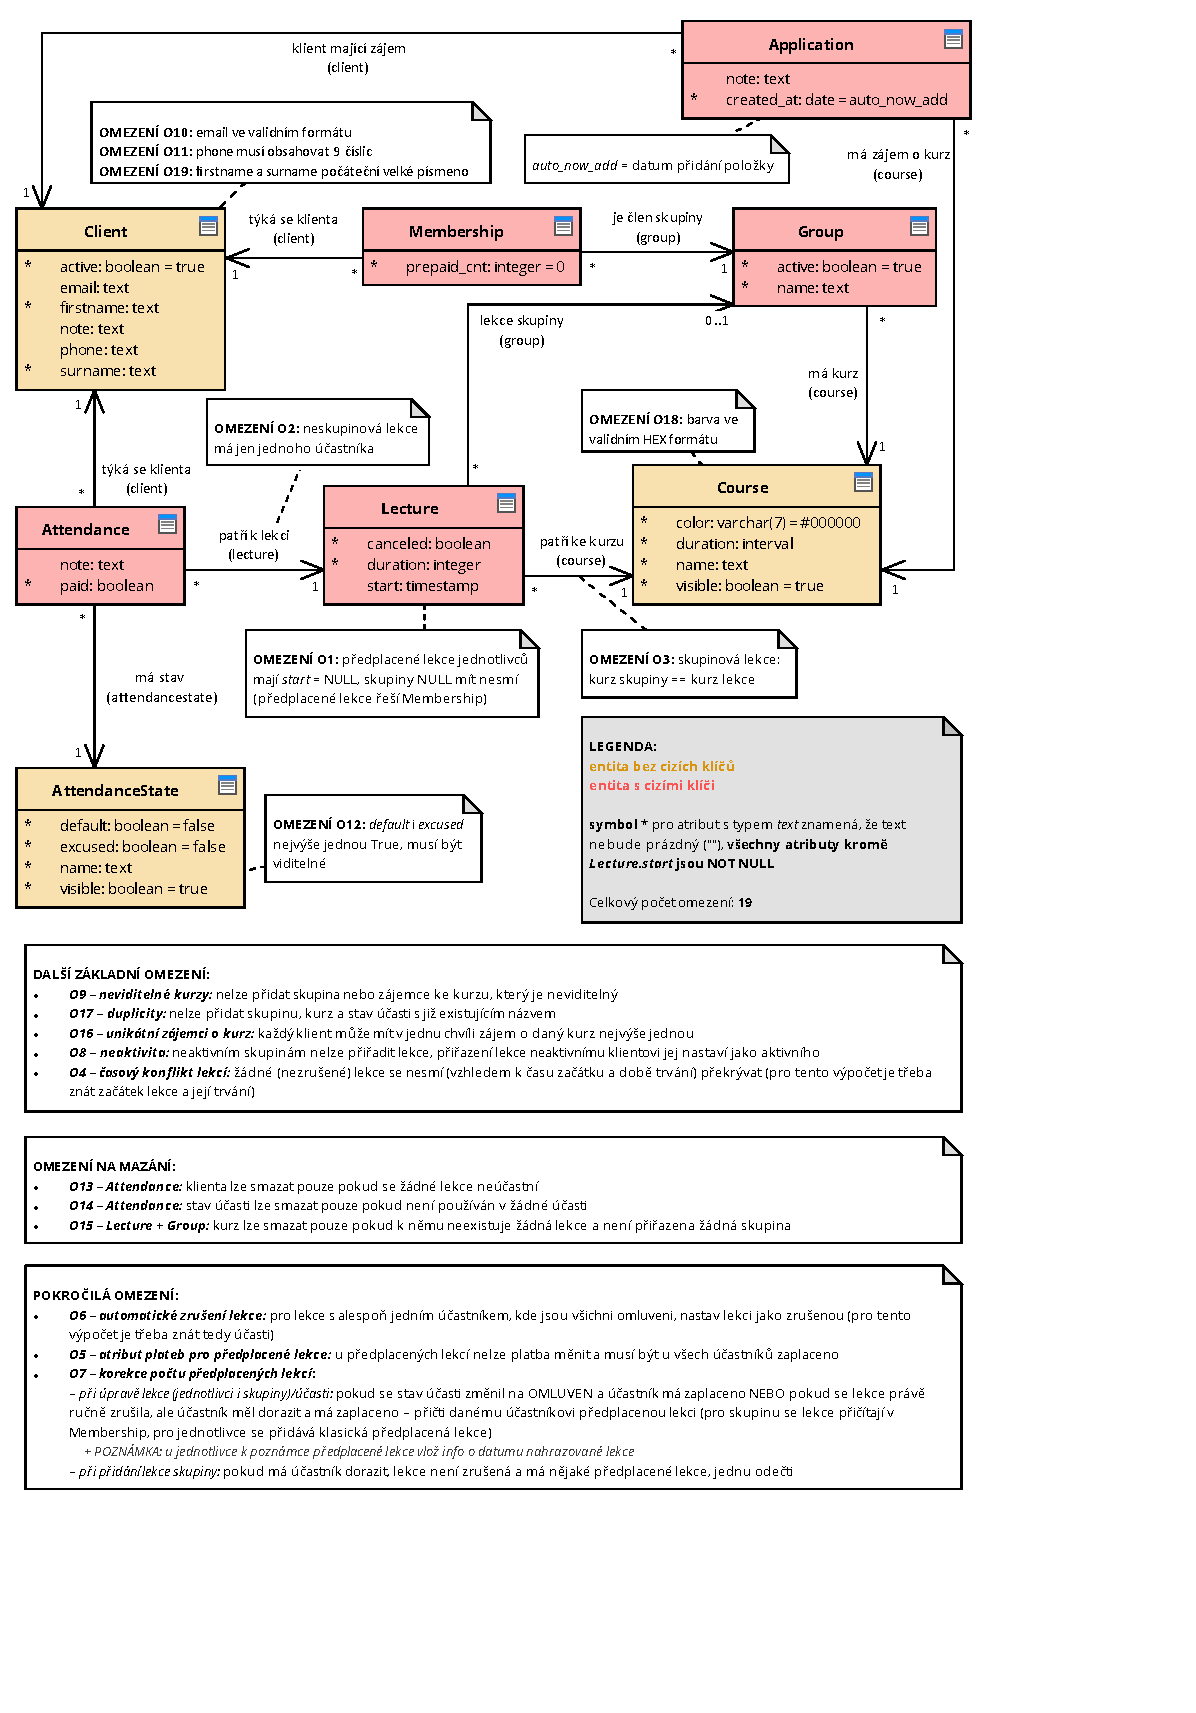
\includegraphics[width=1\textwidth]{img/db-model}
	\caption[Aktualizovaný a rozšířený původní logický datový model]{Aktualizovaný a rozšířený původní logický datový model z~\cite{bp}}\label{fig:db-model}
\vspace{-28pt}
\end{figure}

\subsection{Předplacené lekce}

V předchozím odstavci jsem se dotkl hodnoty \verb|NULL| pro \verb|start| lekce -- zde nastává změna oproti původnímu modelu, protože nyní jsou takto, jak již bylo zmíněno, vedeny pouze předplacené lekce jednotlivců. Díky tomu pak může být u každé předplacené lekce, která se automaticky vytvoří jako náhrada při omluvě/zrušení lekce (viz požadavek~\ref{F10}).

Předplacené lekce skupin jsou pro umožnění jednoduché evidence (viz požadavek~\ref{F3}) nyní součástí členství klientů ve skupině (Membership), tato entita původně byla dekompozicí vztahu M:N bez dalších atributů, prapůvodní záměr v rámci bakalářské práce byl evidování počátku a konce členství klienta ve skupině, což se pak ukázalo jako zbytečné, ale dekompozice byla pro případné jiné budoucí využití ponechána. Nyní tedy konečně dostála svému řádnému využití a umožní tak evidovat počet předplacených lekcí každého klienta v rámci dané skupiny -- když je klient ze skupiny smazán, smaže se samozřejmě i jeho členství a s tím i předplacené skupiny.

\subsection{Zájemci o kurzy}

Dalším funkčním požadavkem~\ref{F1}, který je třeba projevit do datového modelu, jsou zájemci o kurzy. Zde se dá s výhodou jednoduše rozšířit původní datový model o entitu navázanou na klienta a kurz -- tím docílím evidování zájmu klienta o daný kurz (entita Application). Zájem klienta o kurz obsahuje poznámku a také datum přidání, který bude jednoduše automaticky přidávaný, aby lektorka nemusela nic vyplňovat.

\subsection{Vlastnosti stavů účasti}

Požadavek~\ref{F17} uvádí, že je třeba některým stavům přiřadit speciální úlohu -- jeden označit jako výchozí (a zároveň ten, který znamená, že uživatel má přijít/přišel) a druhý jako stav s významem \enquote{klient omluven}. Původní řešení, jak též uvádí \ref{F17}, bylo toto zadefinovat napevno v kódu podle názvu stavu účasti, což je ale nedostačující, protože je samozřejmě třeba tento název umožnit upravit. Nabízelo se několik možností -- zavést nový atribut stavu účasti, který bude označovat typ stavu účasti (jako tomu bývá např. při evidování úrovně oprávnění uživatelů v rámci aplikací). Samotné typy by pak musely být evidovány jako další nová entita. Vzhledem k tomu, že se nepočítá s přidáním dalších typů v budoucnu (stavů účasti také ne, ale ty klidně být přidány mohou, jen nebudou mít speciální typ, protože ten je zde zaveden kvůli dalším speciálním výpočtům jako např. počet absolvovaných lekcí v rámci kurzu), toto řešení nebylo zvoleno z důvodu zbytečné komplexity. Byl zvolen jednodušší způsob, kdy stav účasti má dva boolean atributy \verb|default| a \verb|excused|, kde serverová část obstará, že právě jedna instance stavu účasti bude mít příslušný atribut aktivní. Toto řešení není tak dobře škálovatelné, ale jak jsem uvedl, není to třeba -- je jednoduché a nevyžaduje oproti druhému řešení mnoho změn na úrovni API a klientské části.

\subsection{Další změny}

Aktivita klientů a skupin (viz požadavek~\ref{F6}) se vzhledem k návrhu dá vyřešit jednoduchým atributem \verb|active| u obou těchto entit.

V případě kurzu bylo třeba pro evidování délky trvání kurzu (viz požadavek~\ref{F7}) pro jednotlivce přidat příslušný atribut \verb|duration|. Dalším přidaným atributem je pak \verb|color|, který umožní u kurzu evidovat jeho barvu (viz požadavek~\ref{F12}).

Další změnou, která byla provedena navíc oproti požadavkům bylo přejmenování atributu \verb|name| u klienta na \verb|firstname|. Kromě více vystihujícího názvu (jedná se skutečně o křestní jméno) se zde během vývoje vyskytl problém s nejednoznačností, kde se v rámci klientské části někde pracovalo s \verb|name| jakožto celým jménem klienta, kdežto jinde jako s křestním jménem.

\section{Komunikační rozhraní}

Ukázalo se, že původní komunikační rozhraní (REST API) z bakalářské práce mělo velmi dobrý návrh, bylo třeba provést pouze drobnější úpravy a především začlenit všechny potřebné změny z požadavků a datového modelu. Nejprve se zaměřím na drobnější změny a poté na začlenění změn z požadavků a datového modelu. V rámci této kapitoly nebudu uvádět přesnou novou podobu API včetně původních bodů, ale pouze změny, v rámci požadavku~\ref{N1} totiž bude dostupná dokumentace celého API.

\subsection{Opravy a úpravy stávajícího rozhraní}

Pro odpověď na GET požadavek na lekce (GET \verb|lectures/|) byl u každé účasti klienta klíč \verb|count| pro označení pořadového čísla lekce. Zde jsou dva problémy. Prvním je fakt, že název klíče není úplně přesně vypovídající název vzhledem k dané situaci a při práci v kódu nastávaly nedorozumění, proto došlo k přejmenování na \verb|number|, což lépe odpovídá tomu, že se jedná a pořadové číslo lekce. Druhý problém je, že se z neznámého důvodu tento klíč vyskytoval u každé účasti v rámci lekce, což v případě lekce jednotlivce není důležité, ale v případě skupiny je pak totéž číslo u každé účasti (protože se řeší celkový počet lekcí, nikoliv zda konkrétní klient na nějaké lekci byl) -- tedy zbytečně se informace duplikuje a na klientské části se vezme její první výskyt -- toto bylo opraveno a pořadové číslo lekce se nyní vyskytuje přímo u lekce, nikoliv u každé účasti.

Součástí odpovědi GET \verb|lectures/|, jak již bylo zmíněno, je také přehled účastí jednotlivých klientů, zde bylo rozhodnuto také o odstranění vnořených informací o stavech účasti jednotlivých klientů -- v praxi zde byl poslán vždy název účasti, ID (a nově vzhledem k novému datovému modelu by byly poslány i informace \verb|default| a \verb|excused|), vzhledem k plánovaným změnám v rámci požadavku~\ref{N6} tyto vnořené informace byly odstraněny a nahrazeny pouze ID stavu účasti, protože si klientská část aplikace bude stavy účasti pamatovat (implementace viz TODO).

U klientů, jak bylo uvedeno v datovém modelu v předchozí sekci~\ref{sec:datovymodel}, se přejmenoval klíč pro křestní jméno na \verb|firstname|.
    
\newcommand{\apiA}{0.33}
\newcommand{\apiB}{0.14}
\newcommand{\apiC}{0.43}

\subsection{Předplacené lekce}

Pro lepší evidenci předplacených lekcí jednotlivce (viz požadavek~\ref{F3}) bylo třeba umožnit nějakým způsobem na API zaslat požadavek na přidání daného počtu předplacených lekcí. Nejprve byla zvážena možnost vytváření daného počtu lekcí pomocí zaslání POST požadavku na \verb|lectures/prepaid/| obsahujícím příslušný počet předplacených lekcí, vzhledem k jednodušší implementaci a větší univerzálnosti bylo místo toho umožněno zaslat POST požadavek obsahující více různých lekcí (tedy např. i více předplacených lekcí) na \verb|lectures/|.

Pro lepší evidenci předplacených lekcí skupin je na základě předchozí sekce~\ref{sec:datovymodel} zaveden nový bod \verb|memberhips|. V kódu již byl zaveden serializer pro Membership, ten ale nebude použit, protože by pak bod umožňoval upravovat i ID klienta, kterému členství náleží, což zde není třeba -- bude tedy vytvořen druhý serializer pro Membership, který umožní upravit pouze \verb|prepaid_cnt|. Bod pracuje s klíči \verb|id| a \verb|prepaid_cnt| a jeho podoba je následující:

{\centering
\begin{tabular}{p{\apiA\textwidth} p{\apiB\textwidth} p{\apiC\textwidth}}&&\\
    \verb|memberhips/:id/|     & \textbf{PUT}      & úprava členství s \verb|id|\\
    \verb|memberhips/:id/|     & \textbf{PATCH}    & částečná úprava členství s \verb|id|\\
\end{tabular}}

\subsection{Banka}

Přidání úplně nového bodu nastalo kvůli požadavku~\ref{F8} na zobrazení transakcí z banky -- zde API bude nově umožňovat GET na \verb|bank/|, odpověď bude především obsahovat samotná data z banky, která budou dle potřeba transformována (upravena, doplněna, zjednodušena). Lektorka pro ÚP používá bankovní účet u Fio banky, která nabízí zdarma možnost zřízení přístupu k datům účtu přes API, pomocí získaného tokenu je možné každých 30 sekund zaslat na API požadavek \cite{fioapi}. Vzhledem k tomuto časovému omezení (kde by se jinak lektorka při dalším načtení stránky dočkala chybové hlášky) bylo zde rozhodnuto o cachování získaných dat z banky po dobu 60 sekund.

\subsection{Zájemci o kurzy}

Pro evidenci zájemců o klienty byl též vytvořen nový bod, který pracuje s klíči \verb|id|, \verb|note|, \verb|created_at| a dále obsahuje vnořené informace o kurzu (klíč \verb|course|) a klientovi (klíč \verb|client|). Po vzoru ostatních původních bodů se pro úpravy a vytváření zájemců místo vnořených informací zasílá pouze ID a klíč je ve tvaru \verb|klíč_id| -- tedy \verb|client_id| a \verb|course_id|). Podoba bodu je následující:

{\centering
\begin{tabular}{p{\apiA\textwidth}p{\apiB\textwidth}p{\apiC\textwidth}}&&\\
    \verb|applications/|             & \textbf{GET}      & vrátí všechny zájemce\\
    \verb|applications/|             & \textbf{POST}     & vytvoření nového zájemce\\
    \verb|applications/:id/|         & \textbf{GET}      & vrátí zájemce s \verb|id|\\
    \verb|applications/:id/|         & \textbf{PUT}      & úprava zájemce s \verb|id|\\
    \verb|applications/:id/|         & \textbf{PATCH}    & částečná úprava zájemce s \verb|id|\\
    \verb|applications/:id/|         & \textbf{DELETE}   & smazání zájemce s \verb|id|\\
\end{tabular}}

\subsection{Další rozšíření}

Kvůli požadavku~\ref{F6} pro evidenci aktivních a neaktivních klientů byla pro klienty a lekce zavedena možnost filtrování pomocí query string:
\begin{itemize}
    \item \verb|groups/?active=:boolean|,
    \item \verb|clients/?active=:boolean|.
\end{itemize}

V rámci požadavku~\ref{N6} pro optimalizaci API bylo také přidáno filtrování pro kurzy dle viditelnosti -- \verb|courses/?visible=:boolean|.

Do API bylo také třeba projevit změny z datového modelu v předchozí sekci~\ref{sec:datovymodel}. Pro klienty a skupiny přibyl nový klíč \verb|active| znázorňující aktivitu klienta/skupiny. Pro kurzy byl přidán nový klíč \verb|duration| pro evidování délky trvání kurzu a \verb|color| pro evidování barvy kurzu. Stejně tak zde došlo k projevení změn povinných atributů, povolených hodnota ad., vzhledem k použití Django REST Framework ale není v této oblasti na API provádět v kódu žádné změny, protože se projeví automaticky z datové vrstvy (modelů).

Dále, vzhledem ke zvolenému řešení evidování vlastností stavů účasti v předchozí sekci~\ref{sec:datovymodel} je třeba v bodu \verb|attendancestates/| umožnit pracovat nově i s klíči \verb|default| a \verb|excused|, to je velmi jednoduché (proto byl také tento přístup zvolen).

\section{Architektura}

Aktualizovaný diagram nasazení na obrázku~\ref{fig:deployment-diagram} vychází z původního diagramu \cite{bp}. Jádro zůstává stejné a kromě drobnějších vylepšení pro zlepšení přehlednosti je v něm pouze jedna důležitá změna.
    
\begin{figure}[h]\centering
	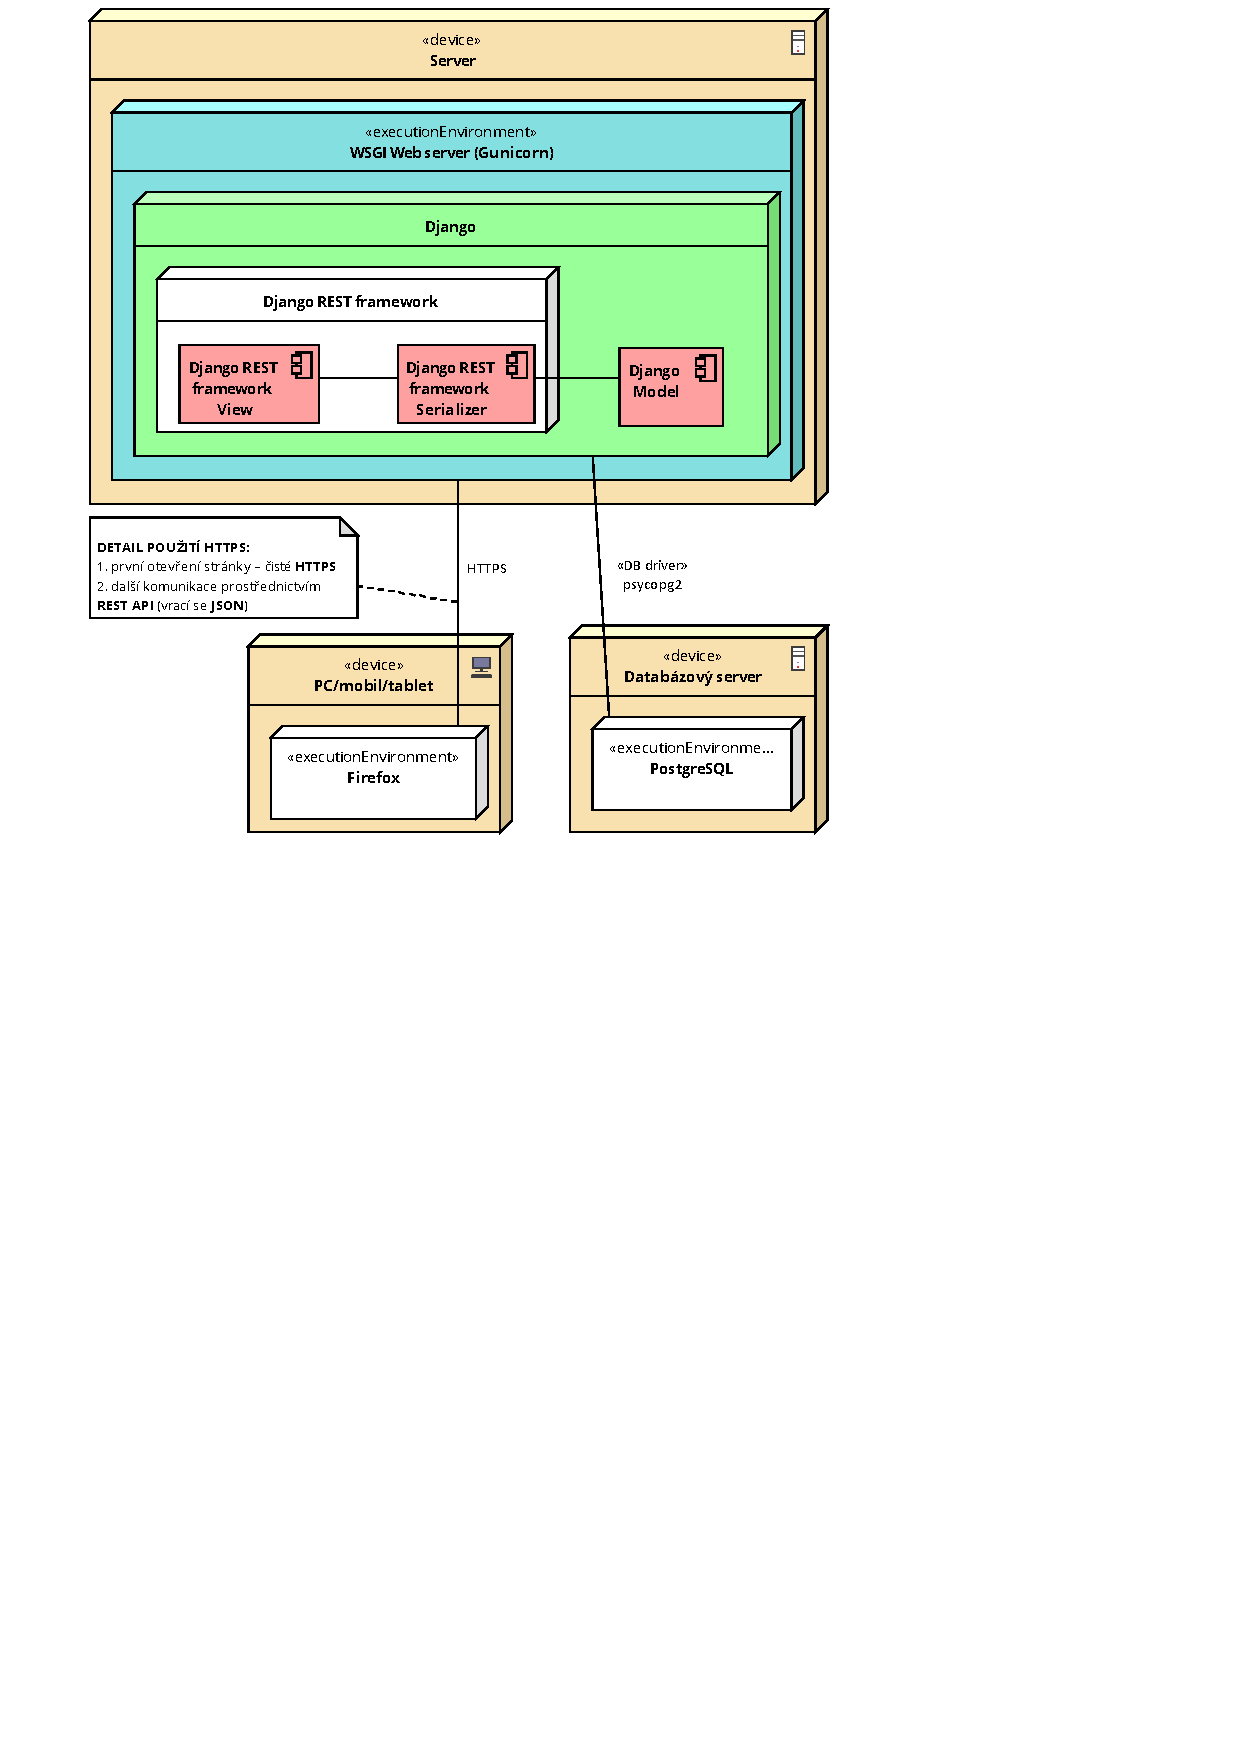
\includegraphics[width=1\textwidth]{img/deployment-diagram}
	\caption[Aktualizovaný diagram nasazení]{Aktualizovaný diagram nasazení, vychází z~\cite{bp}}\label{fig:deployment-diagram}
\end{figure}

V původním diagramu byl jako protokol pro komunikaci mezi serverem a klientem uvedeno HTTP/S. Vzhledem k požadavku na revizi bezpečnosti~\ref{N4} a jeho následné detailní analýze~\ref{subsec:N4detail} je v problému~\ref{B4} zmíněno zavedení HSTS. Podrobnému popisu se budu věnovat v TODO, důležitý je ale dopad na návrh architektury, kde díky zavedení HSTS a korektní konfiguraci aplikace všechna komunikace bude probíhat z důvodu bezpečnosti pouze přes HTTPS (Hypertext Transfer Protocol Secure).

\section{Konfigurace více prostředí}\label{sec:konfiguraceviceprostredi}

V této sekci se budu zabývat návrhem více prostředí pro nasazování aplikace. Nejprve několik úvodních vět pro uvedení do problému. V současnosti je aplikace nasazena pouze v produkčním prostředí (viz popis aktuálního řešení v sekci~\ref{sec:prostreditestovaninasazovani}), kam se automaticky nasazuje při každém úspěchu na CI. V rámci požadavku~\ref{N7} je uvedeno, že je třeba prostředí totožné s produkcí (např. pro reprodukci chyb) a prostředí s aplikací sestavenou na základě poslední revize v repozitáři.

Jak uvádí \cite{deployment-beanstalk}, více prostředí může jít ruku v ruce se vznikem příslušných větví v repozitáři, jejichž názvy odpovídají prostředím, do kterých se nasazují, probíhají zde slučování změn z jednotlivých větví do jiných a poté nasazování do příslušných prostředí. Vzhledem k tomu, že na aplikaci pracuji pouze já, jedná se o aplikaci na míru pro lektorku a nejedná se o obrovský projekt, tento, ač často užívaný postup, jsem se rozhodl zde nezavést. 

Obvyklý vývoj v repozitáři probíhá pomocí vytvoření nové větve s danou novou funkcí, otestování a začlenění změn do hlavní vývojové větve. Některé menší změny jsou případně prováděny rovnou ve výchozí větvi. Na tomto pracovním postupu jsem tedy vytvořil způsob řešení více prostředí, který bude vhodný pro tento projekt na základě požadavku a všech dosavadních znalostech o projektu.

Byl vytvořen návrh více prostředí bez využití příslušných větví:
\begin{itemize}
    \item \textbf{vývojové (lokální):} pro lokální vývoj,
    \item \textbf{testing:} nasazení každé revize (nehledě na větev),
    \item \textbf{staging:} nasazení pro otagované revize, stejná verze aplikace jako produkce,
    \item \textbf{produkce:} nasazení pro otagované revize, aplikace používaná lektorkou.
\end{itemize}

Jakákoliv nová revize (nezávisle na větvi) v repozitáři bude sestavena a automaticky otestována na integračním serveru a nasazena do prostředí \enquote{testing}. Toto prostředí bude velmi podobné produkčnímu, až na verzi aplikace -- jakékoliv změny v aplikaci po provedení \verb|git push| budou tedy vidět nasazené v reálném prostředí -- bude je zde možné pak testovat manuálně jak mnou, tak lektorkou, řešit další úpravy apod. Zde podotknu, že samozřejmě stále zůstává vývojové (lokální prostředí). Až bude vše vyladěno a připraveno na nasazení do produkce, vydá se nová verze aplikace pomocí tagu v gitu (resp. release v GitHubu) -- pak, když tento otagovaný commit dorazí na CI, proběhnou opět též kroky jako v případě běžného commitu, výsledná aplikace bude ale nasazena nejen do prostředí \enquote{testing}, ale také na \enquote{staging} a produkci. Snažím se zde respektovat obecně známé názvy prostředí (jak třeba uvádí \cite{deployment-beanstalk, deployment-oroinc}). Prostředí \enquote{staging} je přesná kopie produkční verze odlišná pouze svou instancí databáze a slouží např. pro reprodukci problémů hlášených z produkce. Produkční prostředí je verze aplikace používaná lektorkou. Díky zmíněnému návrhu se může na produkci nasazovat až v případě, kdy máme vysokou jistotu hladkého běhu na produkci, tedy například po důkladném automatizovaném i manuálním otestování (v závislosti na změnách). Díky zavedení \enquote{staging} prostředí lze snadno reprodukovat problémy mimo produkci, díky \enquote{testing} prostředí lze okamžitě vidět aktuální změny nasazené v reálném prostředí. Navrženému způsobu dodávání nových verzí aplikace se říká průběžné dodávání (CD -- \enquote{Continuous Delivery}) \cite{deployment-atlassian} a jak uvádí \cite{deployment-atlassian}, pro správné fungování CD je třeba mít dostatečně pokrytou aplikaci testy, což řeší požadavek~\ref{N2}.

\section{Uživatelské prostředí}

Do klientské části bylo třeba navrhnout několik prvků z požadavků. Drobnější změny zde ukázány nebudou, zaměřím se jen na nejdůležitější změny v uživatelském rozhraní. Návrhy obvykle probíhaly na papír, ale pro lepší čitelnost je zde uvádím překreslené v aplikaci \href{https://pencil.evolus.vn/}{Pencil}.

\begin{figure}[h]\centering
    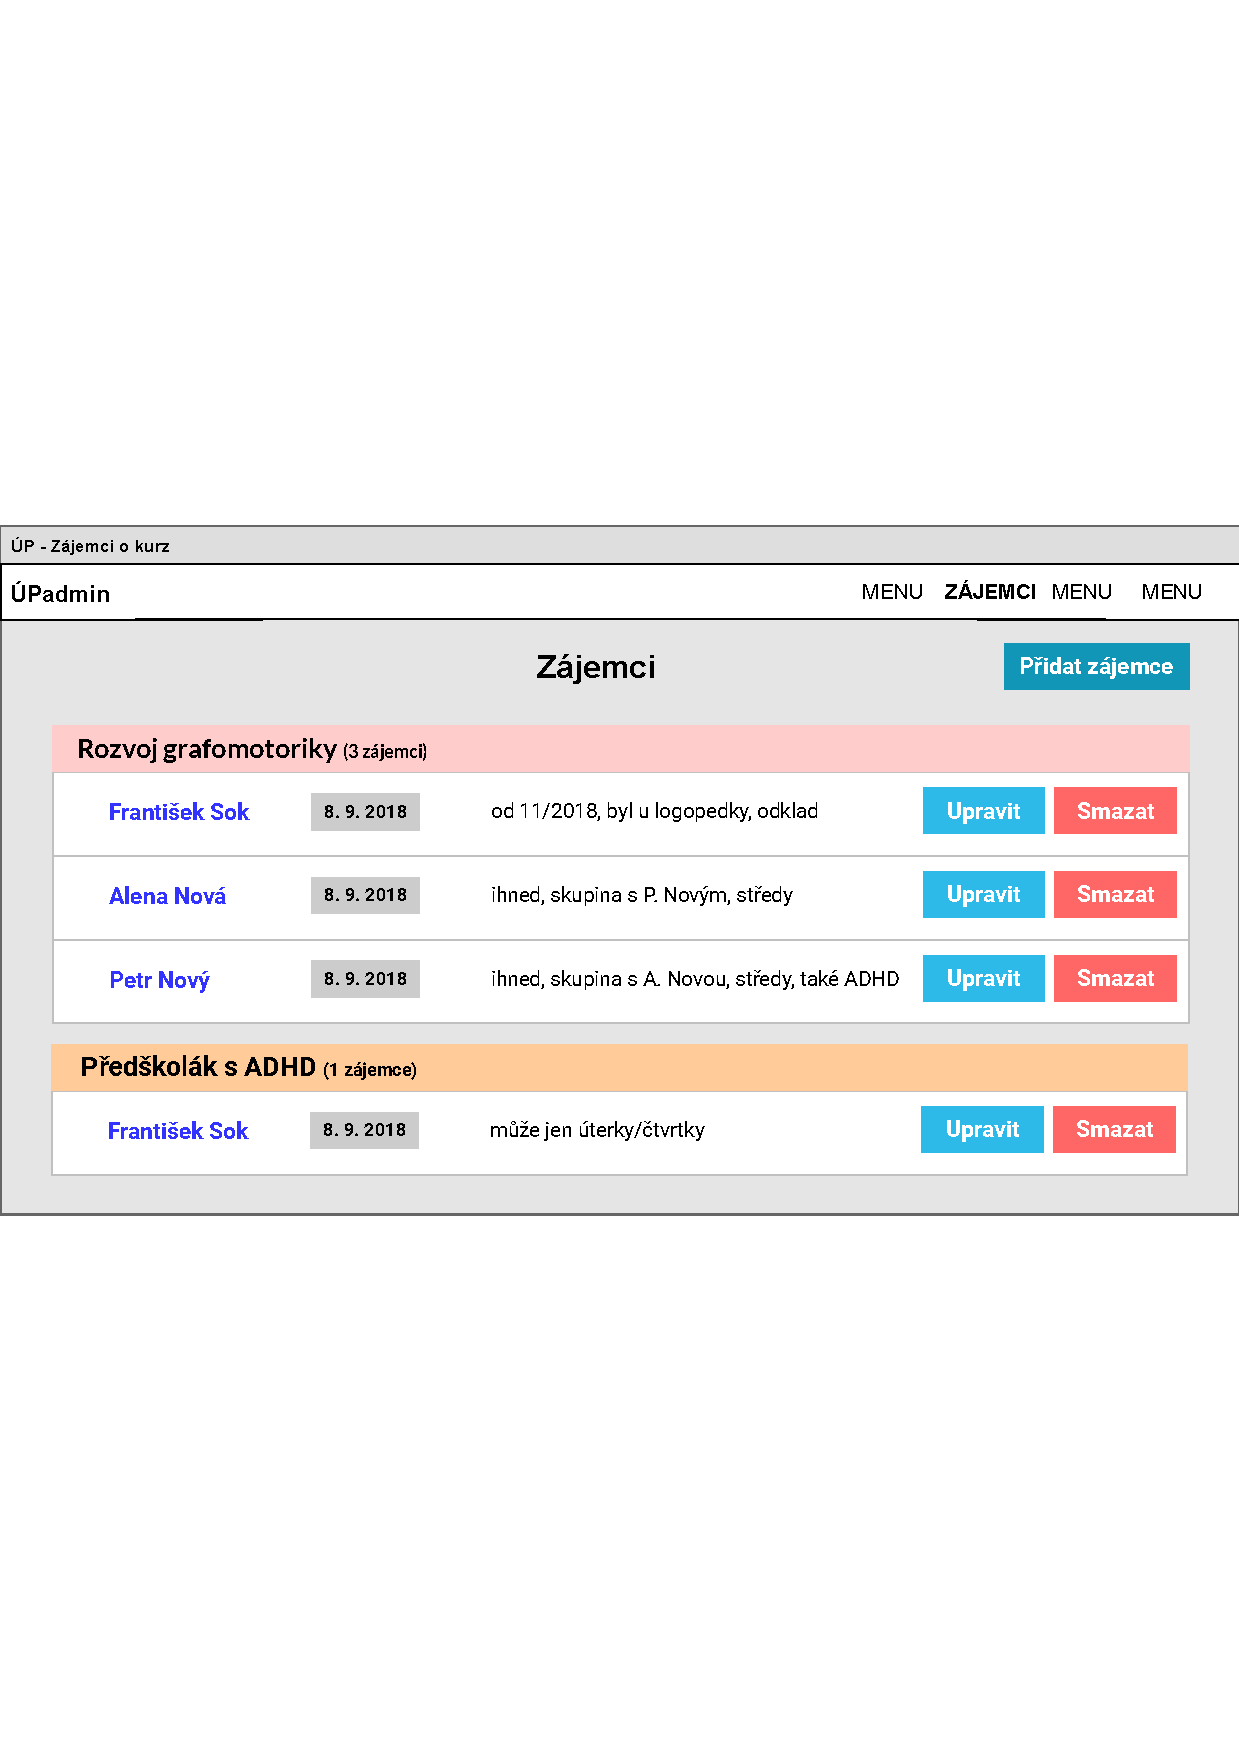
\includegraphics[width=1\textwidth]{img/ui-zajemci}
    \caption{Návrh zájemců o kurzy}\label{fig:ui-zajemci}
\end{figure}

Nejvýraznější změnou v klientské části je přidání nové stránky se zájemci kurzu (viz požadavek~\ref{F1}). Návrh je na obrázku~\ref{fig:ui-zajemci}, jak lze vidět, jsou barevně odlišeny kurzy -- zde již počítám se zavedením požadavku~\ref{F12} pro evidování barev kurzů (změny budou v implementaci učiněny napříč celou aplikací). Návrh splňuje všechny požadavky lektorky, kromě jednoduše dostupné úpravy je také dostupné tlačítko pro smazání -- to je obvykle napříč aplikací dostupné až v modálním okně s úpravou (protože se obvykle stejně nepoužívá a díky tomu, že není přímo na příslušné hlavní stránce, nemůže být ani omylem stisknuto a potvrzeno smazání ve vyskakovacím okně), zde je přímo u každého zájemce, protože oproti ostatním případům zde frekvence mazání bude vysoká vzhledem k postupnému obsluhování všech zájmů o kurzy.

\begin{figure}[h]\centering
    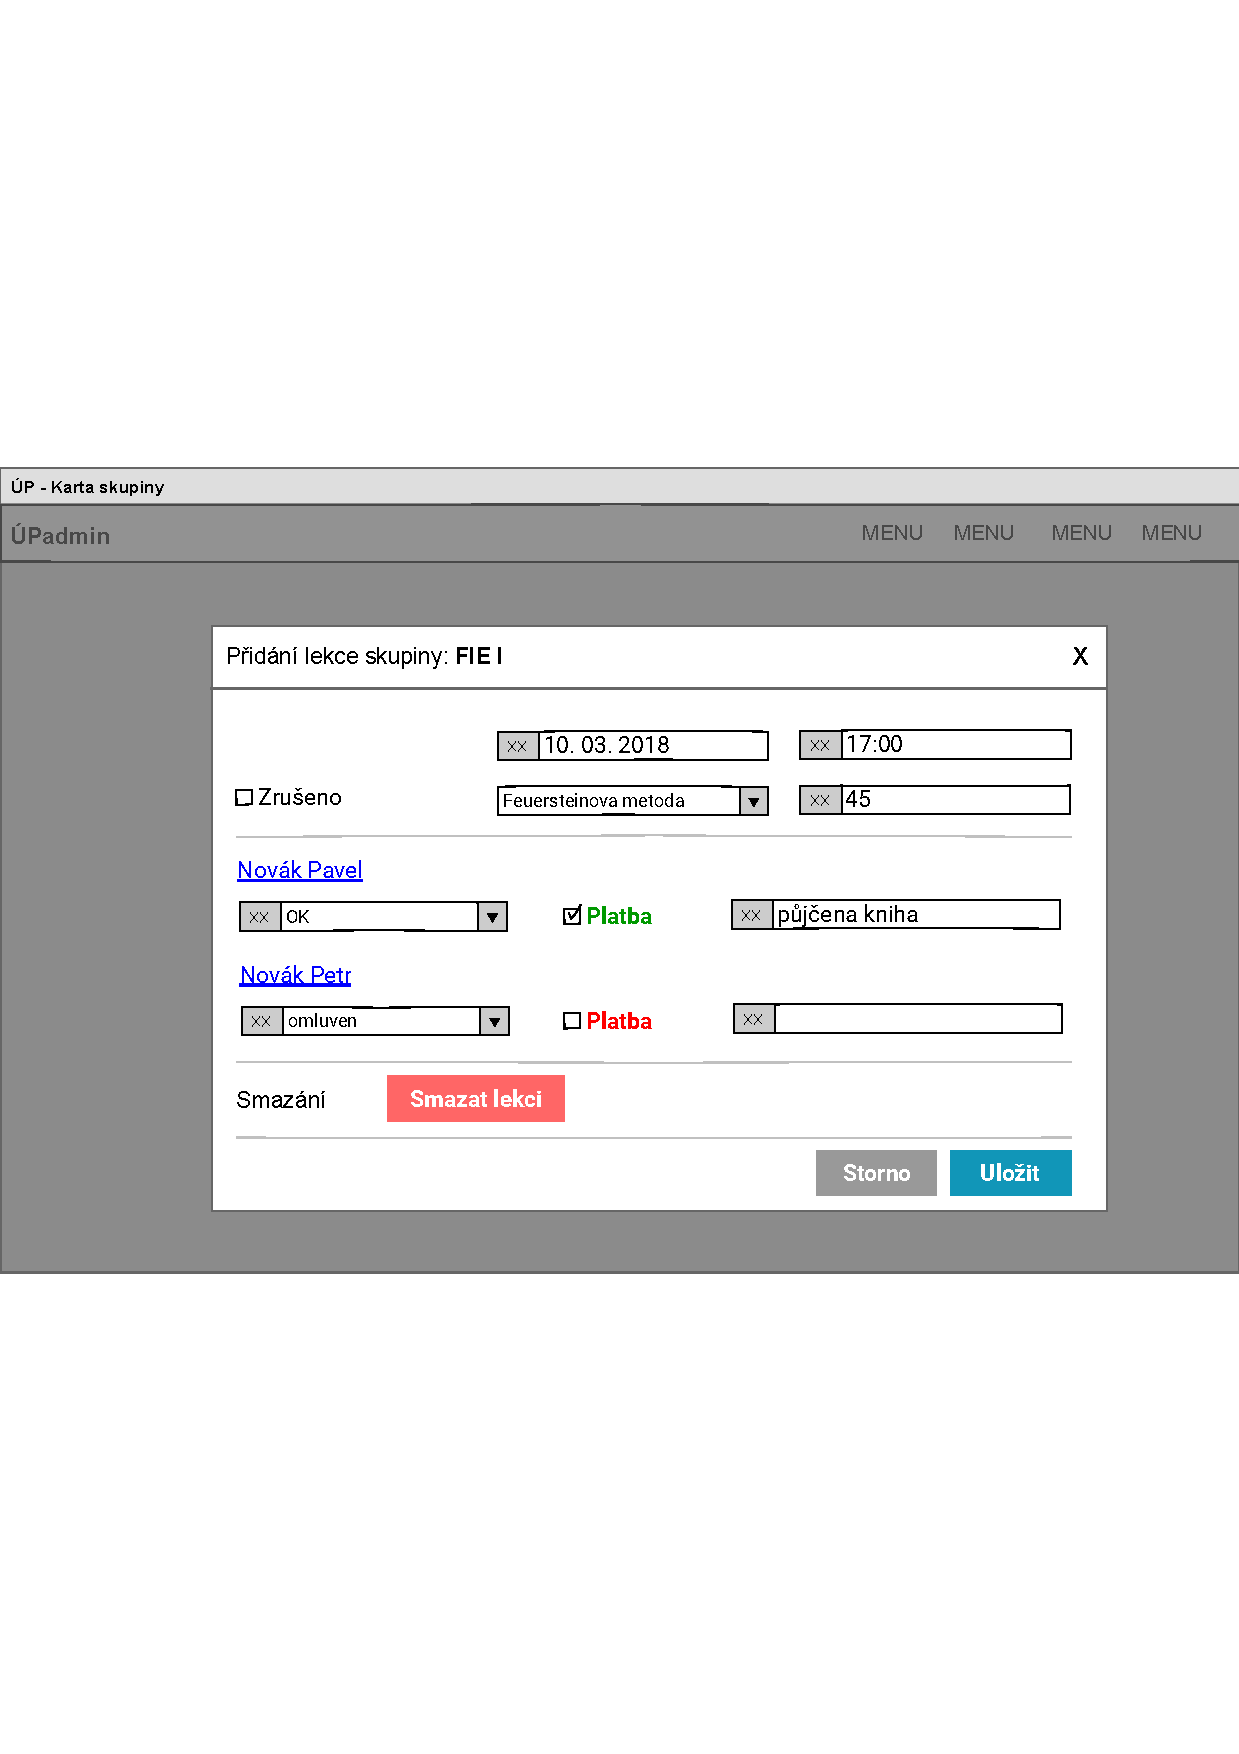
\includegraphics[width=1\textwidth]{img/ui-lekce-skupina}
    \caption{Návrh nového formuláře pro skupinové lekce}\label{fig:ui-lekce-skupina}
\end{figure}

\begin{figure}[ht]\centering
    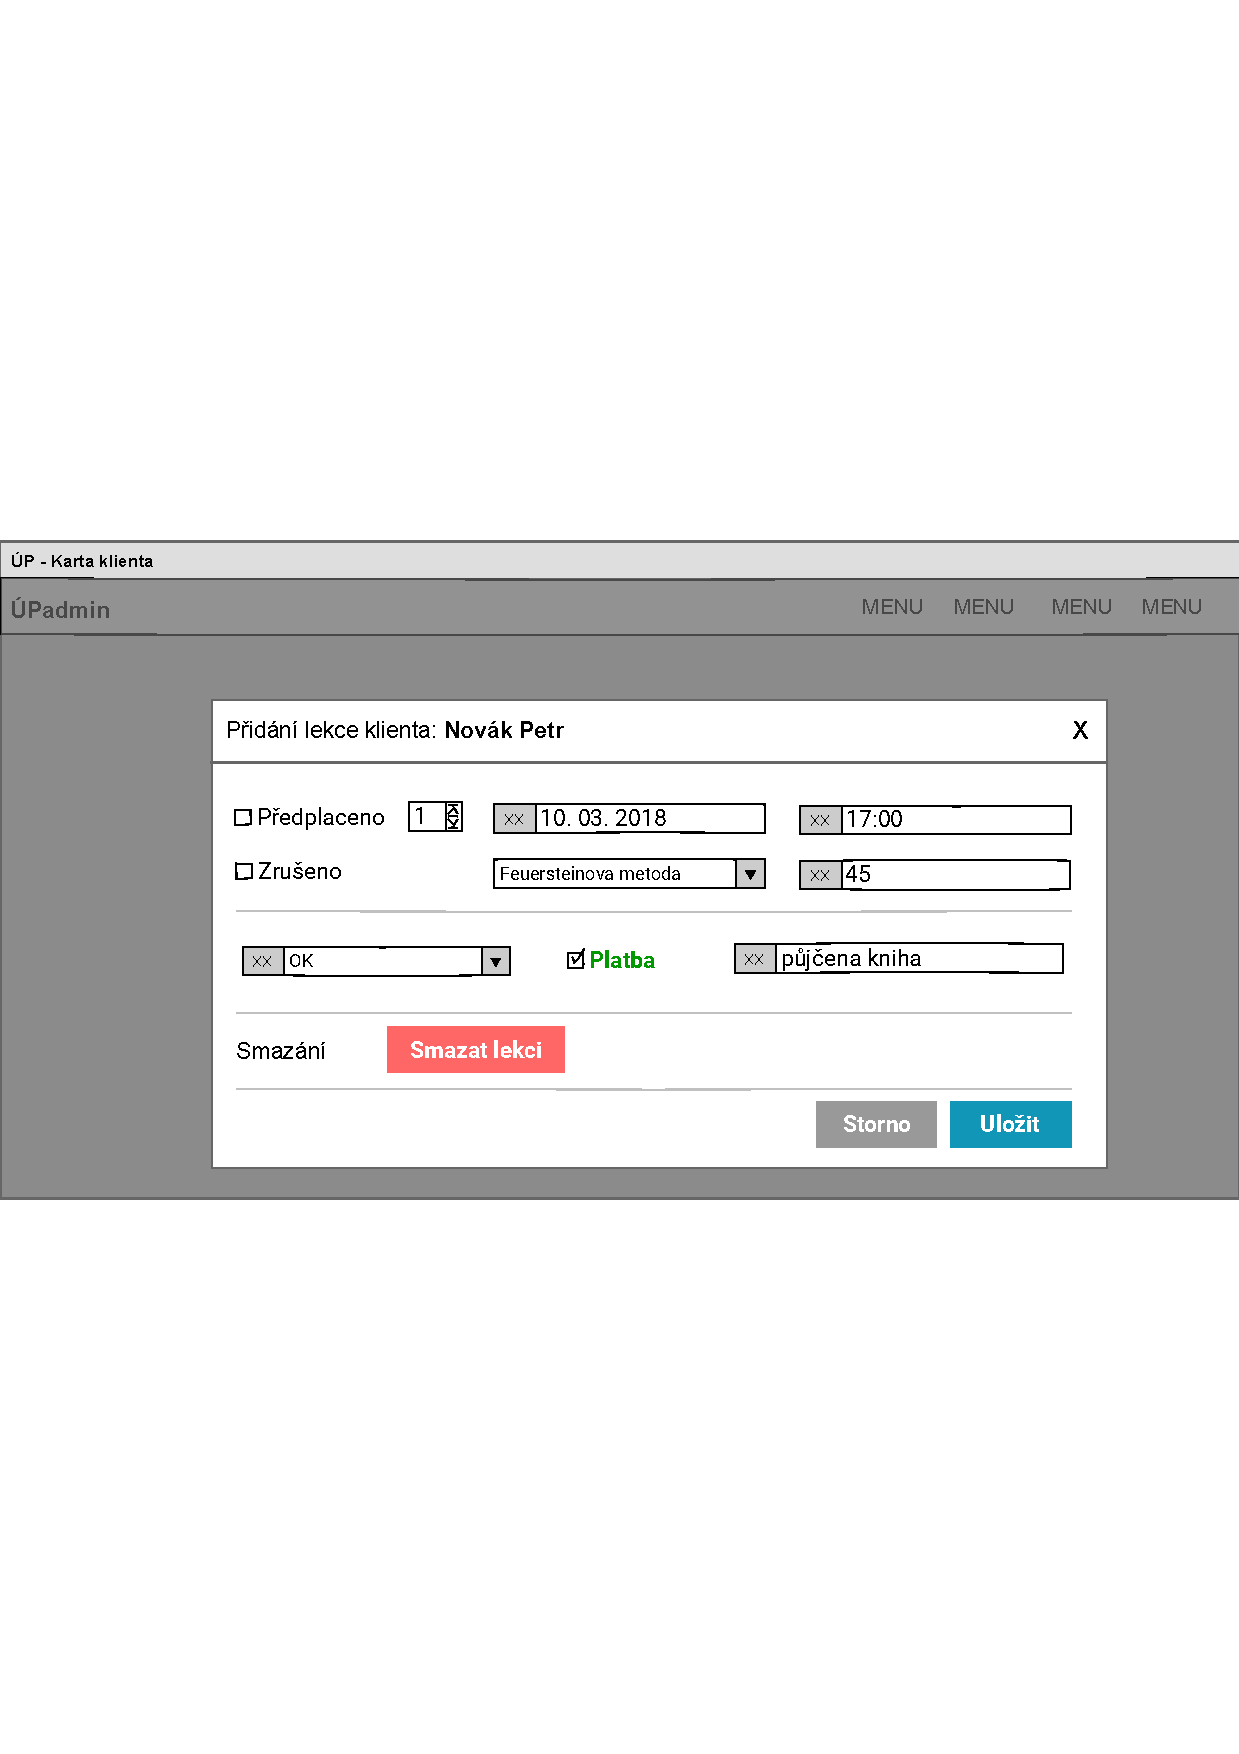
\includegraphics[width=1\textwidth]{img/ui-lekce-klient}
    \caption{Návrh nového formuláře pro lekce jednotlivců}\label{fig:ui-lekce-klient}
\end{figure}

\begin{figure}\centering
    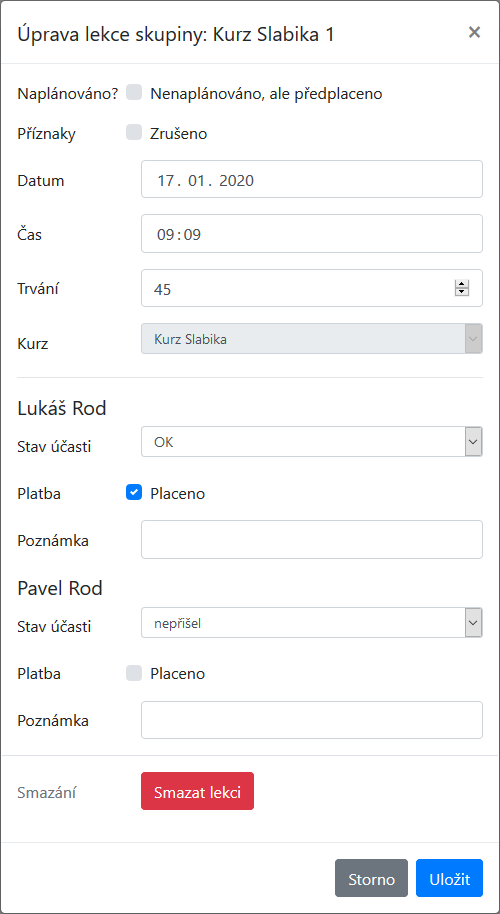
\includegraphics[width=0.55\textwidth]{img/ui-screen-lekce-skupina.png}
    \caption{Původní formulář pro lekce skupin}\label{fig:ui-screen-lekce-skupina}
\end{figure}

Na obrázcích~\ref{fig:ui-lekce-skupina} a \ref{fig:ui-lekce-klient} jsou kompletně přepracované návrhy formulářů pro přidání (a potažmo i úpravu) lekce skupiny, resp. klienta. V rámci příslušného požadavku~\ref{F5} bylo třeba postupnými iteracemi dojít k návrhu, který umožní jednoduší práci s tímto formulářem, který je nejpoužívanější v rámci celé aplikace. V rámci detailní analýzy požadavku~\ref{F3} bylo zjištěno, že je třeba usnadnit přidávání více předplacených lekcí pro jednotlivce, tento požadavek v rámci tohoto přepracování formuláře pro lekce byl též začleněn -- pro klienty je v levém horním rohu dostupné pole pro zapsání počtu předplacených lekcí. Toto pole bude možné upravit při zaškrtnutí volby \enquote{Předplaceno}. Znaky \enquote{XX} u polí naznačují přítomnost ikony vysvětlující význam příslušného pole (místo textů, alternativní text se samozřejmě zobrazí po najetí na ikonu).

Díky větší šířce formuláře bylo možné vměstnat více polí na méně řádků, díky tomu a také ikonám došlo k ušetření místa, díky nově zobrazeným účastem klientů též ve formě řádků, navíc s odlišenou barvou platby je umožněna přehlednější a jednoduší evidence. Jak bylo uvedeno v požadavku~\ref{F5}, jedním z hlavních problémů bylo, že ve skupině může být např. 6 dětí a formulář má pak výšku několika obrazovek a je prakticky nepoužitelný -- zjednodušený názorný příklad původního formuláře (pouze se dvěma účastníky pro jednoduchost, ale účastníků je obvykle mnohem více) je na obrázku~\ref{fig:ui-screen-lekce-skupina}. Formuláře pro skupiny a jednotlivce (klienty) se liší jak počítadlem pro předplacené lekce (u skupin tato možnost není, protože bude řešena počítadly v rámci karty skupiny, viz požadavek~\ref{F3}). Druhou odlišností je pak zobrazení jména účastníka, které v případě jednotlivce je samozřejmě zbytečné (je v horní části formuláře), v případě skupin je toto jméno klienta současně odkazem do jeho karty pro rychlý přechod v případě potřeby.

\chapter{Implementace}


\section{Funkční požadavky}


\subsection{F1 -- evidování zájemců o kurz}


\subsection{F2 -- kontrola časového konfliktu lekcí}


\subsection{F3 -- vylepšení předplacených lekcí}


\subsection{F4 -- vyhledávání klientů}


\subsection{F5 -- přepracování formuláře pro lekce}


\subsection{F6 -- zavedení aktivních a neaktivních klientů a skupin}

* pri uprave/pridani skupiny/klienta dojde automaticky k prepnuti na zalozku aktivni/neaktivni podle toho, do ceho jsme pridavali


\subsection{F7 -- nastavitelná délka kurzů}


\subsection{F8 -- propojení s bankou}

* zobrazují se transakce za posledních 14 dnů, FIO omezuje dotazy na API na 30 s, takže server cachuje odpověď banky rovnou 60 s, zobrazuje se i aktuální zůstatek + barva je podle toho, zda je na účtu dostatek peněz na zaplacení nájmu (zelená, resp. červená s upozorňujícím vykřičníkem s dalšími informacemi), po 60 s možnost výpis obnovit, případně lze jít do bankovnictví, opravuje \#50
* cache, upozorneni na najem


\subsection{F9 -- změny účastníků skupinových lekcí}


\subsection{F10 -- automatické přidání předplacené lekce}


\subsection{F11 -- efektivnější práce v rámci aplikace}


\subsection{F12 -- evidování barev kurzů}


\subsection{F13 -- automatické předvyplnění údajů lekce}


\subsection{F14 -- upozornění na ztrátu dat formulářů}


\subsection{F15 -- vylepšení chybových hlášení}

* frontend odolny proti padu diky ErrorBoundary
* drf zpracovavat ProtectedError https://github.com/rodlukas/UP-admin/issues/70
* podrobnejsi chyby z api
* osetreni v api (IO...)
* notifikace neprekryvaji menu
* osetreni vstupu (vcetne konecne plne funkcniho API)
* js vylepseni notifikaci - notifikace doplnene o nadpis a ikonu, sjednoceny font, komponenta pro obsah notifikace, delsi doba zobrazeni error notifikace
* podrobnější chybové hlášky (např. při ProtectedError, když se uživatel pokouší mazat instanci, na které závisí jiné instance s chráněným příslušným FK; podrobnější info o časovém konfliktu...)


\subsection{F16 -- titulky stránek}


\subsection{F17 -- nastavitelné vlastnosti stavů účasti}


\subsection{F18 -- omezení a validace hodnot}

* pokročilá validace duplicit apod.
* zruseni noveho omezeni "neaktivní klienty nelze přiřadit do skupin (UI je ani nezobrazí ve výběru)" - neaktivní klienti již mohou být členové skupiny
* velka pocatecni pismena jmena klienta i pro api, presun transformaci field z modelu do serializeru
* viz EA docs
* js zvyrazneni neaktivity skupin a klientu napric aplikaci https://github.com/rodlukas/UP-admin/issues/85


\subsection{F19 -- automatické zrušení lekce}


\subsection{F20 -- zobrazení zrušených lekcí}


\subsection{F21 -- skupinové lekce bez účastníků}



\section{Nefunkční požadavky}


\subsection{N1 -- dokumentace}


\subsection{N3 -- zavedení nástrojů pro usnadnění vývoje a údržby}

* refaktoring
* js komponenta pro zobrazeni lekci https://github.com/rodlukas/UP-admin/issues/71
* template strings js
* python refaktoring https://github.com/rodlukas/UP-admin/issues/93
* zavedeni prvnich hooku, drobna vylepseni komponent - prechod na funkcionalni komponenty, upravy komponent (napr. zbytecne pouzivaly stav nebo se zbytecne casto updatovaly, ikdyz to nebylo potreba) + **odstranění zbytečného stavu odstranilo i chybu, která byla už od počátku v aplikaci a způsobovala občasné nefungování komponenty s aktuálním stavem účasti - zobrazil se jiný stav, než byl skutečný, v závislosti na pořadí obdržení odpovědí od serveru, to se začalo víc projevovat při nedávných změnách architektury reactu**
* opravy nekonzistentnich stavu
* analyza pruchodu aplikaci (google analytics)
* opravy nevalidniho html a css (diky tomu lepsi zarovnani tlacitek)
*  js useEffect - exhaustive deps https://github.com/rodlukas/UP-admin/issues/96
* prechod na TS: dalsi zmeny viz https://github.com/rodlukas/UP-admin/releases/tag/1.0.0
* Minifikace HTML
* oprava práce se setState - zbytečně se přes const state = this.state nastavoval pak ve setState celý nový stav, což je zbytečné a navíc to může způsobovat problémy při dalším volání setState (které když proběhne před tímto, může přijít v niveč, protože jej nahradí tato kompletní změna stavu, ačkoliv se má měnit jen malá část stavu komponenty) 



podrobny popis jak probihalo zavedeni, co mi to umoznuje, treba i screenshoty, k cemu to bylo pouzito, jak se to osvedcilo - nastroje vychazi ze zvolenych nastroju z reserse


LGTM: 
[js] odstraneni unused promenne v Applications
[js] oprava spatneho nazvu promenne v inicializaci ErrorBoundary
[js] oprava potencialnich chyb zpusobenych nespravnou aktualizaci stavu
[python] odstraneni vsech import *
[python] optimalizace importu
[js] optimalizace importu
[js] oprava primeho zapisovani do stavu v Card
[js] konzistentni stav PrepaidCounters
[js] konzistentni stav at\_state ve FormLecture

sonarcloud viz commity koment


sider PR
houndCI PR
codefactor nefunkcni dependence stylelint, eslint config js nepodporuje
code-inspector - katastrofalni UI, naprosto nefunkcni parsovani, importy nefunguji... (v UI nefunguje ani tlacitko zpet a vse je rozpadle...)


deepcode
deepscan, sonarcloud, lgtm
deepsource
codebeat
codeclimate
codacy

\begin{itemize}
\item ...
\item code formatting - prettier, black
\item python zavedeni vulture pro dead code
\item napojeni na Sentry, Slack, logentries, GA
\item zavedeni LGTM, opravy nalezenych problemu
\item travis: zavedeni cache pro yarn a pipenv, zjednoduseni prace s .npmrc, na heroku se neprovadi build a collectstatic
\item zmena react toolkitu (nejdrive nwb, pak test neutrinojs a nakonec custom webpack + porovnani size bundle), viz https://github.com/rodlukas/UP-admin/issues/67 a https://github.com/rodlukas/UP-admin/issues/65
\item ...
\end{itemize}

\subsection{N4 -- revize bezpečnosti}

* contextapi pro prihlasovani - zmeny viz https://github.com/rodlukas/UP-admin/releases/tag/0.8


\subsection{N5 -- vylepšení použitelnosti}


\subsection{N6 -- optimalizace API}

* DRF-JWT problémy, dotazy na SQL DB ikdyž nemají být - https://github.com/rodlukas/UP-admin/issues/51 - přechod na jinou knihovnu a zde PR na překlad do CZ
* viditelne kurzy api, dalsi filtrovani (aktivita)
* pomalé SQL dotazy- obri optimalizace dotazu na DB (>4x zrychleni) diky DJDT, pokrocile optimalizace
* odstraneni zbytecne prace s DB napric api - zrychleni - commit https://github.com/rodlukas/UP-admin/commit/ba12eea6be642d0c56629ac607fb1f8ffab267f7
* vice info viz https://github.com/rodlukas/UP-admin/releases/tag/0.9.0



%součástí sekce bude i sypani popela na hlavu za chyby v bakalarce - popisu co vsechno se delo, co bylo za problemy (napr bad patterny v reactu, coz zpusobilo ruzne problemy)

\begin{comment}

% todo migrace na novy react

PR:
* chyby při práci s modálními okny https://github.com/rodlukas/UP-admin/issues/95 - issue reactstrapu, vyjde nova verze
* react fontawesome PR pro vylepseni typescript podpory (ID atribut..)
* reactstrap tooltip ios fix


* "noopener noreferrer" z důvodu bezpečnosti
* robots.txt, pak nahrazeni robots.txt meta tagem pro uplny zakaz cehokoliv robotum
* pipfile
* mnoho promennych prostredi → ve všech prostředích se pracuje stejným způsobem s příslušnými proměnnými prostředí, je čistější nastavení Djanga a umožňuje díky .env souboru (je v .gitignore) použít i lokální proměnné prostředí (jinak těžko univerzálně nastavitelné i v rámci IDE) + odstranění zašifrovaných proměnných v konfiguráku travisu a přesun přímo do repo
* zobrazení tel. čísel klientů v zájemcích o kurz (\#61)
* oprava logiky výpočtu "příště platit" - nebral v úvahu předplacené lekce (https://github.com/rodlukas/UP-admin/commit/e84aa4eec9bb93323a097830dd1416204658c87a)
* lekce je automaticky zrušená na frontendu i backendu když jsou všichni účastníci omluveni, na to je příslušně uživatel upozorněn ve formuláři (a zároveň zrušení nejde měnit, protože by backend lekci stejně tak či tak zrušil)
* rozdělení CSS stylů ke komponentám
* asynchronní update všech dní v týdnu v diáři při nějaké změně (ca53c16), opravuje \#19
* zjednodušení kódů a struktury souborů, refactoring, odstranění všech zbytečných getDerivedStateFromProps (nahrazeno např. componentDidUpdate)
* migrace na nový životní cyklus komponent Reactu (503b9ac)
* funkční zobrazení vývojové verze na jiném zařízení v síti
* oprava chyby způsobující nekorektní zobrazení lekcí v předchozím dnu - když např. byla lekce v 1 h ráno, v diáři se ukázala v předchozím dni jako poslední → porovnávávání datumu s TZ s datumem bez TZ → vyřešeno použitím "\_\_date" v querysetu (3da9db1)
* oprava chybné práce s datumem v diáři (JS) - pokud se zadala URL s datumem, kde den měl číslo "31", došlo k "přesunu do minulosti" (číslo dne se změnilo na "1") - v důsledku toho se v aplikaci nedalo dostat do roku 2019, protože 31.12.2018 bylo pondělí a další týden se přepnul na listopad
* 05-2019 prechod na nwb
* mene pozadavku - react context api (attendancestates + nově také viditelné kurzy, aktivní klienti/skupiny - vše napříč aplikací) -> TÍM PÁDEM POTŘEBA PŘEJÍT NA NOVÝ REACT -> je tedy potřeba provést i migraci na nový lifecycle reactu, vice viz https://github.com/rodlukas/UP-admin/releases/tag/0.8
* redesign vsech stranek pro lepsi konzistenci, srozumitelnost a pochopeni (predelany diar, zajemci, lekce v karte...)
* Pro zrychlení načítání celé aplikace se používá lazy loading React.lazy + React Suspense - umozni kratsi prvni nacteni appky, zalozene na react-routeru + reseni nastaleho problemu -- reseni Error: Loading chunk 11 failed. https://github.com/rodlukas/UP-admin/issues/92
* optimalizace frontendu - odstraneni komponent definovanych primo v render - mohlo zpusobit potize s vykonem i nechtenym prekreslovanim vnorenych komponent
* úprava stavových kódu API pro bankovnictví (\#55) - už vrací jen 200/500, ostatní chyby jsou zahrnuty v 500 a podrobnější informace jsou přiloženy do JSONu rovnou na serveru (tedy na frontendu není žádná logika navíc)
* úpravy a opravy API - na backendu nechybí žádná logika, která doteď mohla být třeba i jen na frontendu - už fungují všude PATCH metody, kód API je rozumnější, efektivnější a přehlednější a nedělají se v něm zbytečné kraviny navíc, rozumně se např. už pracuje i s takovými atributy, které lze zaslat na API jako null, ošetření všech možných případů - opravuje \#52

    kompletní validace tel. čísla na backendu i frontendu, vylepšení způsobu validace a dělení čísla na mezery už při psaní o formuláře, následné odstranění mezer až na backendu
    oprava chyby způsobující chybu při úpravě stavu účasti předplacené lekce
* odstranění křížku pro reset react-selectu, aby nedocházelo k vymazání "omylem", když funkcionalita stejně není třeba
* občas se využívají skupinové lekce bez definovaných účastníků (ještě nejsou známí), taková lekce se ale ukazuje jako zrušená a u skupiny chybí info, že nejsou žádní účastníci - potřeba vylepšit zobrazení

\end{comment}


\chapter{Testování}
pozadavek N2
implementace samotneho testovani v behave, Selenium

https://www.katalon.com/resources-center/blog/continuous-testing-introduction/

N2: 
* vylepseni vsech testu - neprobihala kontrola zobrazenych dat ve formulari pred upravou
* zrychleni testu upravy klientu
* vylepseni potvrzovani formulare pro lepsi zachyceni chyb
* oprava náhodně občas nefungujících testů na CI (po každém scénáři je smazána localstorage) (\#64)

\begin{itemize}
\item popis, jak jsem konkretne tvoril vsechny UI/API testy v behave a seleniu, co bylo za problemy (nacitani, viz heuristika), jak to funguje, jak jsem vsechno udelal
\item coverage 86 \%
\item popsat co vsechno se testuje, ze je to v jazyku gherkin
\item popsat co se netestuje
\item pripadne zminit ze bylo reseno v ramci MI-PYT
\item popsat dalsi problemy s nehezkym API selenia, ktere je pro ruzne jazyky nejednoznacne a nesjednocene (mozna kvuli verzi 3, v4 uz asi bude lepsi...), hrozna dokumentace, ale zase to pouzivaj vsichni tak se vsechno vsude najde
\item pripadne dodat akceptacni testovani
\item niels. heur. analyza, ktera pomohla pak v implementaci prakticky zprovoznit UI testovani, protoze co nevi clovek, nevi ani selenium a tezko se neco testuje (nevi ze se nacita kdyz to nevidi ani clovek, nevi ze se ma cekat..)
\item mozna zminit usability testovani - zejmena proto, ze prakticky na tom stoji dalsi vylepseni v analyze, kde jsem pozoroval lektorku pri bezne praci a na zaklade toho jsme resili, co by chtela zmenit/pridat/upravit; tady neni treba testovat pro jine uzivatele, je to zamerene na interni pouziti 1 clovekem, o to lepsi to ale musi byt:)
\end{itemize}


\chapter{Nasazení}
pozadavky N7,N8
popis toho jak jsem udelal novej zpusob nasazovani
* django-environ

\section{Zavedení více prostředí}
\begin{itemize}
\item vyvoj BP probihal na lokalu a pak probehl push na GH, travis provedl build a testy a nasadilo se na produkci, to znamená že jsem samozřejmě produkci mohl zbořit (a taky že párkrát zbořil..)
\item jak funguje stage, testing, produkce, demo co kam kdy jde v souvislosti s releasy, k cemu to je, jak se to osvedcilo - dohledavani problemu na stage kdyz se neco stane na produkci
\item (zustava dev a produkce)
\item pokročilé debugování na lokálním i vzdáleném prostředí díky Django Debug Toolbar 
\item vyhoda testing a demo env je ze tam muze kdokoliv, neuvidi nic duverneho (ani pristup do banky tu neni povolen), takze do toho muze vedouci prace, oponent i bezny uzivatel, da se testovat vse na obdobnem prostredi jako pak bude staging, produkce (heroku)
\item + samozrejme je zde moznost spustit na lokalu, ale todle je mnohem rychlejsi (viz GH)
\end{itemize}

\section{Další úpravy}
\begin{itemize}
\item automaticke zalohovani DB
\item ...
\end{itemize}



\chapter{Možná rozšíření}
klasika - co by se dalo delat dal, o co by se appka mohla rozsirit, dalsi technologie, fce

\chapter{Zveřejnění jako open-source}
repo na GH uz je pripravene: https://github.com/rodlukas/UP-admin - vcetne instrukci pro spusteni
\begin{itemize}
\item popsat proc zverejnit - moznost nahlednout na realnou aplikaci s nejnovejsimi technologiemi, jak je nakonfigurovana, inspirovat se + ma reference
\item MIT licence
\item popsat co bylo treba pro zverejneni udelat - priprava vsech casti, vyreseni tokenu, promennych prostredi... + problem: automaticky zverejneni buildu frontendu, aby ho clovek mohl pouzit pri spusteni u sebe na lokalu - protoze se pouziva placena knihovna, ke ktere mam pristup jen ja, takze si to nikdo jiny u sebe nezbuildi (resi to travis a nahraje build do assetu k release) - řešení: na travisu se provede build frontendu a ten se automaticky jako *zip* soubor nahraje k příslušnému github release 
\item na GH  je popsání vlastností, požadavků, postupu instalace a spuštění, testování + připravená vzorová data pro DB (včetně návodu na jejich vložení)
\item (? promenne prostredi mozna zminim i jinde)
\end{itemize}




        
    \bookmarksetup{startatroot} % aby nasledujici kapitoly nespadaly do partu s praktickou casti
    \addtocontents{toc}{\bigskip}
    
    \begin{conclusion}
    	TODO
    \end{conclusion}
    
    \printbibliography
    \appendix
    
    \chapter{Seznam použitých zkratek} %TODO
        % \printglossaries
        \begin{description}
            \item[API] Application Programming Interface
            \item[AJAX] Asynchronous JavaScript and XML
            \item[CBA] Component-Based Architecture
            \item[CMS] Content Management System
            \item[CRM] Customer Relationship Management
            \item[CRUD] create-read-update-delete
            \item[CSR] Client-Side Rendering
            \item[CSRF] Cross-Site Request Forgery
            \item[CSS] Cascading Style Sheets
            \item[DRF] Django REST Framework
            \item[DRY] Don\textquotesingle t repeat yourself
            \item[GUI] Graphical User Interface
            \item[HTML] Hypertext Markup Language
            \item[HTTP] Hypertext Transfer Protocol
            \item[IaaS] Infrastructure as a Service
            \item[JS] Javascript
            \item[JSON] JavaScript Object Notation
            \item[MVC] Model-view-controller
            \item[MVP] Model-view-presenter
            \item[MVT] Model-view-template
            \item[MVW] Model-view-whatever
            \item[MPA] Multi-Page Application
            \item[ORM] Object-Relational Mapping
            \item[PaaS] Platform as a Service
            \item[SEO] Search Engine Optimization
            \item[SPA] Single-Page Application
            \item[SQL] Structured Query Language
            \item[SSR] Server-Side Rendering
            \item[UI] User Interface
            \item[URL] Uniform Resource Locator
            \item[ÚP] Úspěšný prvňáček
            \item[UX] User Experience
            \item[XML] eXtensible Markup Language
            \item[XSS] Cross-Site Scripting
        \end{description}
    
    \chapter{Obsah přiloženého DVD} %TODO
        \begin{figure}
        	\dirtree{%
        		.1 readme.txt\DTcomment{stručný popis obsahu DVD}.
        		.1 src.
        		.2 impl\DTcomment{zdrojové kódy implementace}.
        		.2 thesis\DTcomment{zdrojová forma práce ve formátu \LaTeX{}}.
        		.1 text\DTcomment{text práce}.
        		.2 rodlukas{\_}dp.pdf\DTcomment{text práce ve formátu PDF}.
        	}
        \end{figure}
\end{document}
